\documentclass{article}
\usepackage[backend=biber,natbib=true,style=alphabetic,maxbibnames=50]{biblatex}
\addbibresource{/home/nqbh/reference/bib.bib}
\usepackage[utf8]{vietnam}
\usepackage{tocloft}
\renewcommand{\cftsecleader}{\cftdotfill{\cftdotsep}}
\usepackage[colorlinks=true,linkcolor=blue,urlcolor=red,citecolor=magenta]{hyperref}
\usepackage{amsmath,amssymb,amsthm,enumitem,float,graphicx,mathtools,tikz}
\usetikzlibrary{angles,calc,intersections,matrix,patterns,quotes,shadings}
\allowdisplaybreaks
\newtheorem{assumption}{Assumption}
\newtheorem{baitoan}{Bài toán}
\newtheorem{cauhoi}{Câu hỏi}
\newtheorem{conjecture}{Conjecture}
\newtheorem{corollary}{Corollary}
\newtheorem{dangtoan}{Dạng toán}
\newtheorem{definition}{Definition}
\newtheorem{dinhly}{Định lý}
\newtheorem{dinhnghia}{Định nghĩa}
\newtheorem{example}{Example}
\newtheorem{ghichu}{Ghi chú}
\newtheorem{goal}{Goal}
\newtheorem{hequa}{Hệ quả}
\newtheorem{hypothesis}{Hypothesis}
\newtheorem{lemma}{Lemma}
\newtheorem{luuy}{Lưu ý}
\newtheorem{nhanxet}{Nhận xét}
\newtheorem{notation}{Notation}
\newtheorem{note}{Note}
\newtheorem{principle}{Principle}
\newtheorem{problem}{Problem}
\newtheorem{proposition}{Proposition}
\newtheorem{question}{Question}
\newtheorem{remark}{Remark}
\newtheorem{theorem}{Theorem}
\newtheorem{vidu}{Ví dụ}
\usepackage[left=1cm,right=1cm,top=5mm,bottom=5mm,footskip=4mm]{geometry}
\def\labelitemii{$\circ$}
\DeclareRobustCommand{\divby}{%
	\mathrel{\vbox{\baselineskip.65ex\lineskiplimit0pt\hbox{.}\hbox{.}\hbox{.}}}%
}
\setlist[itemize]{leftmargin=*}
\setlist[enumerate]{leftmargin=*}

\title{Lecture Note: Combinatorics {\it\&} Graph Theory\\Bài Giảng: Tổ Hợp {\it\&} Lý Thuyết Đồ Thị}
\author{Nguyễn Quản Bá Hồng\footnote{A scientist- {\it\&} creative artist wannabe, a mathematics {\it\&} computer science lecturer of Department of Artificial Intelligence {\it\&} Data Science (AIDS), School of Technology (SOT), UMT Trường Đại học Quản lý {\it\&} Công nghệ TP.HCM, Hồ Chí Minh City, Việt Nam.\\E-mail: {\sf nguyenquanbahong@gmail.com} {\it\&} {\sf hong.nguyenquanba@umt.edu.vn}. Website: \url{https://nqbh.github.io/}. GitHub: \url{https://github.com/NQBH}.}}
\date{\today}

\begin{document}
\maketitle
\begin{abstract}
	This text is a part of the series {\it Some Topics in Advanced STEM \& Beyond}:
	
	{\sc url}: \url{https://nqbh.github.io/advanced_STEM/}.
	
	Latest version:
	\begin{itemize}
		\item {\it Lecture Note: Combinatorics \& Graph Theory -- Bài Giảng: Tổ Hợp \& Lý Thuyết Đồ Thị}.
		
		PDF: {\sc url}: \url{https://github.com/NQBH/advanced_STEM_beyond/blob/main/combinatorics/lecture/NQBH_combinatorics_graph_theory_lecture.pdf}.
		
		\TeX: {\sc url}: \url{https://github.com/NQBH/advanced_STEM_beyond/blob/main/combinatorics/lecture/NQBH_combinatorics_graph_theory_lecture.tex}.
		\item {\it Slide: Combinatorics \& Graph Theory -- Slide Bài Giảng: Tổ Hợp \& Lý Thuyết Đồ Thị}.
		
		PDF: {\sc url}: \url{https://github.com/NQBH/advanced_STEM_beyond/blob/main/combinatorics/slide/NQBH_combinatorics_graph_theory_slide.pdf}.
		
		\TeX: {\sc url}: \url{https://github.com/NQBH/advanced_STEM_beyond/blob/main/combinatorics/slide/NQBH_combinatorics_graph_theory_slide.tex}.
		\item {\it Survey: Combinatorics \& Graph Theory -- Khảo Sát: Tổ Hợp \& Lý Thuyết Đồ Thị}.
		
		PDF: {\sc url}: \url{https://github.com/NQBH/advanced_STEM_beyond/blob/main/combinatorics/NQBH_combinatorics.pdf}.
		
		\TeX: {\sc url}: \url{https://github.com/NQBH/advanced_STEM_beyond/blob/main/combinatorics/NQBH_combinatorics.tex}.
		\item Codes:
		\begin{itemize}
			\item C{\tt/}C++: \url{https://github.com/NQBH/advanced_STEM_beyond/blob/main/combinatorics/C++}.
			\item Pascal: \url{https://github.com/NQBH/advanced_STEM_beyond/blob/main/combinatorics/Pascal}.
			\item Python: \url{https://github.com/NQBH/advanced_STEM_beyond/blob/main/combinatorics/Python}.
		\end{itemize}
	\end{itemize}
\end{abstract}
\tableofcontents

%------------------------------------------------------------------------------%

\section*{Preliminaries}

\subsection*{Notation -- Ký hiệu}

\begin{itemize}
	\item $\overline{m,n}\coloneqq\{m,m + 1,\ldots,n - 1, n\}$, $\forall m,n\in\mathbb{Z}$, $m\le n$. Hence the notation ``for $i\in\overline{m,n}$'' means ``for $i = m,m + 1,\ldots,n$'', i.e., chỉ số{\tt/}biến chạy $i$ chạy từ $m\in\mathbb{Z}$ đến $n\in\mathbb{Z}$. Trong trường hợp $a,b\in\mathbb{R}$, ký hiệu $\overline{a,b}\coloneqq\overline{\lceil a\rceil,\lfloor b\rfloor}$ có nghĩa như định nghĩa trước đó với $m\coloneqq\lceil a\rceil,n\coloneqq\lfloor b\rfloor\in\mathbb{Z}$; khi đó ký hiệu ``for $i\in\overline{a,b}$'' với $a,b\in\mathbb{R}$, $a\le b$ có nghĩa là ``for $i = \lceil a\rceil,\lceil a\rceil + 1,\ldots,\lfloor b\rfloor - 1,\lfloor b\rfloor$, i.e., chỉ số{\tt/}biến chạy $i$ chạy từ $\lceil a\rceil$ đến $\lfloor b\rfloor\in\mathbb{Z}$.
	\item $\lfloor x\rfloor,\{x\}$ lần lượt được gọi là {\it phần nguyên \& phần lẻ} (integer- \& fractional parts) của $x\in\mathbb{R}$, see, e.g., \href{https://en.wikipedia.org/wiki/Floor_and_ceiling_functions}{Wikipedia{\tt/}floor \& ceiling functions}, \href{https://en.wikipedia.org/wiki/Fractional_part}{Wikipedia{\tt/}fractional part}.
	\item $x_+\coloneqq\max\{x,0\}$, $x_-\coloneqq\max\{-x,0\} = -\min\{x,0\}$ lần lượt được gọi là {\it phần dương \& phần âm} (positive- \& negative parts) của $x\in\mathbb{R}$.
	\item s.t.: abbreviation of `such that'.
	\item w.l.o.g.: abbreviation of `without loss of generality'.
	\item $|A|$ or $\#A$: the number of elements of a set $A$ -- số phần tử của 1 tập hợp $A$ hữu hạn.
	\item ${\rm card}(A)$: cardinality of a set $A$ (finite or infinite) -- lực lượng của 1 tập hợp $A$ (hữu hạn hoặc vô hạn).
	\item $[n]\coloneqq\{1,2,\ldots,n\}$: the set of 1st $n\in\mathbb{N}^\star$ positive integers, which serves as 1 of prototypical example of a finite set with $n$ elements -- tập hợp $n\in\mathbb{N}^\star$ số nguyên dương  đầu tiên, đóng vai trò là 1 trong ví dụ nguyên mẫu của một tập hợp hữu hạn với $n$ phần tử. Quy ước $[0] = \emptyset$ ký hiệu tập rỗng, i.e., tập hợp không chứa bất cứ phần tử nào.
	\item $A_n^k$: Chỉnh hợp chập $k$ phần tử từ 1 tập hợp có $n$ phần tử.
	\item $C_n^k = \binom{n}{k}$: Tổ hợp chập $k$ phần tử từ 1 tập hợp có $n$ phần tử.
	\item $P_n = n!$, $\forall n\in\mathbb{N}$: the number of permutations.
	\item O: Olympiad problem -- Bài tập định hướng ôn luyện Olympic Toán Hoặc Olympic Tin.
	\item R: Research-oriented problems -- Bài tập định hướng nghiên cứu.
\end{itemize}

%------------------------------------------------------------------------------%

\section{Basic Combinatorics -- Tổ Hợp Cơ Bản}
Combinatorics is a collection of techniques \& a language for the study of (finite or countably infinite) discrete structures. Given a set of elements (\& possibly some structure on that set), typical questions in combinatorics are:
\begin{itemize}
	\item Does a specific arrangement of the elements exist?
	\item How many such arrangements are there?
	\item What properties do these arrangements have?
	\item Which 1 of the arrangements is maximal, minimal, or optimal according to some criterion?
\end{itemize}
-- Tổ hợp là một tập hợp các kỹ thuật \& một ngôn ngữ để nghiên cứu các cấu trúc rời rạc (hữu hạn hoặc vô hạn đếm được). Cho một tập hợp các phần tử (\& có thể có một số cấu trúc trên tập hợp đó), các câu hỏi điển hình trong tổ hợp là:
\begin{itemize}
	\item Có tồn tại sự sắp xếp cụ thể của các yếu tố không?
	\item Có bao nhiêu sự sắp xếp như vậy?
	\item Những sự sắp xếp này có những tính chất gì?
	\item Sự sắp xếp nào là tối đa, tối thiểu hoặc tối ưu theo một số tiêu chí?
\end{itemize}

%------------------------------------------------------------------------------%

\subsection{Set theory}
\textbf{\textsf{Resources -- Tài nguyên.}}
\begin{enumerate}
	\item \cite{Halmos1960,Halmos1974}. {\sc Paul Richard Halmos}, {\it Naive Set Theory}.
	
	{\sf Comments.} 1 trong những quyển sách có nội dung đẹp nhất về Lý Thuyết Tập Hợp Ngây Thơ (distinguish Naive Set Theory vs. Axiomatic Set Theory -- Lý Thuyết Tập Hợp Tiên Đề).
	\item \cite{Kaplansky1972,Kaplansky1977}. {\sc Irving Kaplansky}. {\it Set Theory \& Metric Spaces}.
\end{enumerate}
Tập hợp là 1 khái niệm cơ bản của Toán học, thường không định nghĩa trong naive set theory (nhưng có thể trong axiomatic set theory). Thông thường, người ta dùng khái niệm tập hợp để chỉ 1 nhóm các đối tượng đã được chọn ra, hay đã được quy định từ trước, \& thường dùng ký hiệu tập hợp bằng chữ in hay chữ viết hoa $A,B,C,X,Y,Z$, tuy nhiên, nên viết ký hiệu bao hàm ý nghĩa của tập hợp để tiện theo dõi trong nghiên cứu, e.g., $\mathbb{N}_{\rm odd} = \{n\in\mathbb{N};n\not{\divby}\ 2\}$: tập hợp các số tự nhiên lẻ, $\mathbb{N}_{\rm even} = \{n\in\mathbb{N};n\divby2\}$: tập hợp các số tự nhiên chẵn. Cho tập $A$, 1 đối tượng $x$ được nói đến trong $A$ được gọi là 1 {\it phần tử} của $A$, ký hiệu $x\in A$, nếu $x$ không nằm trong A, nói $x$ không thuộc $A$, ký hiệu $x\notin A$.
\begin{itemize}
	\item {\it Quy ước.} Tập rỗng $\emptyset$ là tập hợp không gồm phần tử nào cả. Tập $\emptyset$ là duy nhất (uniqueness of emptyset: {\it the} emptyset).
	\item {\it Đo độ lớn của tập hợp.} Khi tập $A$ có hữu hạn phần tử thì số phần tử của $A$ ký hiệu là $|A|$ hoặc $\#A$ hoặc ${\rm card}\,A$ (cardinal -- lực lượng).
	\item {\it2 cách đặt{\tt/}xác định tập hợp.}
	\begin{itemize}
		\item Liệt kê các phần tử của tập hợp.
		\item Chỉ ra tính chất đặc trưng của các phần tử của tập hợp.
	\end{itemize}
\end{itemize}

\begin{remark}[Tính phân biệt của các phần tử trong cùng 1 tập hợp]
	Tập hợp gồm các phần tử phân biêt nhau, i.e., nếu $A = \{a_1,\ldots,a_n\}\Rightarrow a_i\ne a_j$, $\forall i,j = 1,\ldots,n$, $i\ne j$.
\end{remark}

\begin{dinhnghia}[Subset -- Tập con]
	Cho 2 tập $A,B$. $A\subset B\Leftrightarrow(\forall x\in A\Rightarrow x\in B)$: $A$ là {\rm tập con} của $B$, hay $B$ là {\rm tập mẹ} của $A$, ký hiệu $B\supset A$.
\end{dinhnghia}

\begin{dinhnghia}[2 tập hợp bằng nhau]
	(i) 2 tập hợp bằng nhau: $A = B\Leftrightarrow(A\subset B\land B\subset A)$. (ii) Cho $n\in\mathbb{N}$, $n\ge2$, $n$ tập hợp bằng nhau: $A_1 = A_2 = \cdots = A_n\Leftrightarrow A_i = A_j,\ \forall i,j = 1,\ldots,n\Leftrightarrow(A_i\subset A_j\land A_j\subset A_i),\ \forall i,j = 1,\ldots,n$.
\end{dinhnghia}

\begin{theorem}[Some basic properties of sets \& operations on sets -- Vài tính chất cơ bản của tập hợp \& các phép toán trên tập hợp]
	Let $n\in\mathbb{N}^\star$, $A,B,C,\ldots,A_i$ be sets, $\forall i = 1,\ldots,n$.
	\item(i) {\rm(Tính chất của tập con)} $A\subset B\land B\subset C\Rightarrow A\subset C$. $\emptyset\subset A\subset A$, $\forall$ set $A$.
	\item(ii) (Reflective) $A = A$, $\forall$ set $A$. (Symmetric) $A = B\Rightarrow B = A$. (Transitive) $A = B\land B = C\Rightarrow A = C$. $(|A| = |B|\land A\subset B)\Rightarrow A = B$.
\end{theorem}

\begin{dinhnghia}[Giao của 2 tập hợp]
	{\rm Giao} của 2 tập hợp $A,B$ được cho bởi $A\cap B = \{x;x\in A\land x\in B\}$.
\end{dinhnghia}

\begin{dinhnghia}[Hợp của 2 tập hợp]
	{\rm Hợp} của 2 tập hợp $A,B$ được cho bởi $A\cup B = \{x;x\in A\lor x\in B\}$.
\end{dinhnghia}

\begin{dinhnghia}[Hiệu của 2 tập hợp]
	{\rm Hiệu} của 2 tập hợp $A,B$ được cho bởi $A\backslash B = \{x;x\in A\land x\notin B\}$.	
\end{dinhnghia}

\begin{dinhnghia}[Phần bù của 2 tập hợp]
	Cho $A\subset B$. {\rm Phần bù} của $A$ trong $B$ là tập $\overline{A} = B\backslash A$ hay $C_B^A = B\backslash A$.
\end{dinhnghia}

\begin{dinhnghia}[Tích Descartes, \cite{Phuong_to_hop}, p. 12]
	Cho $n\in\mathbb{N}^\star$ tập họp $A_1,\ldots,A_n$. Xét tập hợp $A$ gồm tất cả các bộ $n$ phần tử sắp thứ tự $(a_1,\ldots,a_n)$ trong đó $a_i\in A_i$, $\forall i = 1,\ldots,n$. Tập $A$ được gọi là {\rm tích Descartes} của $n$ tập hợp $A_1,\ldots,A_n$ \& ký hiệu:
	\begin{equation*}
		A = \prod_{i=1}^n A_i = A_1\times A_2\times\cdots\times A_n = \{(a_1,\ldots,a_n);a_i\in A_i,\ \forall i = 1,\ldots,n\}.
	\end{equation*}
\end{dinhnghia}

\begin{dinhly}[Tính chất của tích Descartes]
	(i) $A\times B\ne B\times A$, $\forall A\ne B$. (ii) $|\prod_{i=1}^n A_i| = \prod_{i=1}^n |A_i|$.
\end{dinhly}
A {\it multiset} is like a set except that its members need not be distinct.

-- 1 {\it đa tập hợp} giống như một tập hợp ngoại trừ các thành viên của nó không cần phải khác biệt.

\begin{definition}[Multisets, \cite{Shahriari2022}, Def. 2.13, p. 53]
	A {\rm multiset} is a set together with a function that assigns a positive integer or $\infty$ -- called a {\rm repetition number} (or a {\rm multiplicity}) -- to each member of the set.
\end{definition}

\begin{dinhnghia}[Đa tập]
	Một {\rm đa tập} là một tập hợp cùng với một hàm gán một số nguyên dương hoặc $\infty$ -- được gọi là {\rm số lặp lại} (hoặc {\rm bội số}) -- cho mỗi phần tử của tập hợp.
\end{dinhnghia}

\begin{example}[\cite{Shahriari2022}, Ex. 2.14, p. 53]
	$A = \{a,a,a,b,c,c,d,d\} = \{3\cdot a,b,2\cdot c,2\cdot d\}$ is a multiset with members $a,b,c,d$ \& with repetitions numbers $3,1,2,2$, resp.
\end{example}

\begin{remark}[\cite{Shahriari2022}, Rmk. 2.15, p. 53]
	A set can be thought of as a multiset with all repetitionn numbers equal to 1. In an infinite multiset, some members could have infinite repetition numbers. I.e., we allow for the possibility that a multiset contains an infinite number of copies of a certain element.
	
	-- Một tập hợp có thể được coi là một đa tập hợp với tất cả các số lặp lại bằng 1. Trong một đa tập hợp vô hạn, một số phần tử có thể có số lặp lại vô hạn. Tức là, chúng ta cho phép khả năng một đa tập hợp chứa một số lượng vô hạn các bản sao của một phần tử nhất định.
\end{remark}

\begin{definition}[$|\cdot|$ notation]
	If $X$ is a finite set, then $|X|$ will denote the number of elements in $X$. If $X$ is a finite multiset, then $|X|$ will denote the sum of its repetition numbers.
\end{definition}

\begin{dinhnghia}[Ký hiệu $|\cdot|$]
	Nếu $X$ là một tập hợp hữu hạn, thì $|X|$ sẽ biểu thị số phần tử trong $X$. Nếu $X$ là một đa tập hữu hạn, thì $|X|$ sẽ biểu thị tổng số lần lặp lại của nó.
\end{dinhnghia}

\begin{baitoan}[\cite{Phuong_to_hop}, VD3, p. 16]
	Cho $a,b\in\mathbb{N}^\star$ thỏa $a + b$ lẻ. Chia $\mathbb{N}^\star$ thành 2 tập rời nhau $A,B$ (được gọi là {\rm phân hoạch}). Chứng minh luôn tồn tại 2 phần tử $x,y$ thuộc cùng 1 tập thỏa $|x - y|\in\{a,b\}$.
\end{baitoan}

\begin{baitoan}[\cite{Phuong_to_hop}, VD4, p. 17, [MOSP1997]
	Phân hoạch $\mathbb{N}^\star$ thành $A,B$. Chứng minh $\forall n\in\mathbb{N}^\star$, tồn tại $a,b\in\mathbb{N}^\star$, $a\ne b$, $a > n$, $b > n$ thỏa $\{a,b,a + b\}\subset A$ hoặc $\{a,b,a + b\}\subset B$.
\end{baitoan}

\begin{baitoan}[\cite{Phuong_to_hop}, VD5, p. 19]
	Cho $A\subset[15]$ thỏa tích của 3 phần tử khác nhau bất kỳ của $A$ đều không phải là số chính phương. (a) Chỉ ra 1 tập $A$ gồm $10$ phần tử. (b) Xác định số phần tử lớn nhất của $M$.
\end{baitoan}

\begin{baitoan}[\cite{Phuong_to_hop}, 3., p. 20]
	Cho các tập $A_1,\ldots,A_n$ thỏa $A_i\ne A_j$, $\forall i,j = 1,\ldots,n$, $i\ne j$. Chứng minh có ít nhất 1 tập hợp $A_i$ không chứa tập nào trong các tập còn lại.
\end{baitoan}

\begin{baitoan}[\cite{Phuong_to_hop}, 4., p. 20]
	(a) Cho tập $A\subset\mathbb{R}$ thỏa đồng thời: (i) $\mathbb{Z}\subset A$. (ii) $\sqrt{2} + \sqrt{3}\in A$. (iii) $x + y\in S,xy\in S$, $\forall x,y\in S$. Chứng minh $\dfrac{1}{\sqrt{2} + \sqrt{3}}\in A$. (b) Mở rộng giả thiết (ii) thành $\sqrt{n} + \sqrt{n + 1}$, $\forall n\in\mathbb{N}^\star$. Chứng minh $\dfrac{1}{\sqrt{n} + \sqrt{n + 1}}\in A$. (c) Mở rộng giả thiết (ii) thành $\sqrt{a} + \sqrt{b}$, $\forall a,b\in\mathbb{N}^\star$, $a\ne b$. Chứng minh $\dfrac{(a - b)^2}{\sqrt{a} + \sqrt{b}}\in A$. (d) Mở rộng giả thiết (ii) thành $\sqrt[3]{a} + \sqrt[3]{b}$, $\forall a,b\in\mathbb{Z}$, $a\ne b$. (e) Mở rộng giả thiết (ii) thành $\sqrt[n]{a} + \sqrt[n]{b}$, $\forall a,b\in\mathbb{Z}$, $a\ne b$, với $n\in\mathbb{N}$, $n\ge2$ cho trước.
\end{baitoan}

\begin{proof}
	(a) $\sqrt{2} + \sqrt{3}\in A\xRightarrow{\rm(iii)}(\sqrt{2} + \sqrt{3})^2 = 5 + 2\sqrt{6}\in A\xRightarrow[-5\in\mathbb{Z}\subset A]{\rm(iii)}2\sqrt{6}\in A\xRightarrow{\rm(iii)}2\sqrt{6}(\sqrt{2} + \sqrt{3}) = 4\sqrt{3} + 6\sqrt{2}\in A\Rightarrow\dfrac{1}{\sqrt{2} + \sqrt{3}} = \sqrt{3} - \sqrt{2} = 5(\sqrt{2} + \sqrt{3}) - (4\sqrt{3} + 6\sqrt{2})\in A$.
	
	\item(b) $\sqrt{n} + \sqrt{n + 1}\in A\xRightarrow{\rm(iii)}(\sqrt{n} + \sqrt{n + 1})^2 = 2n + 1 + 2\sqrt{n(n + 1)}\in A\xRightarrow[-(2n + 1)\in\mathbb{Z}\subset A]{\rm(iii)}2\sqrt{n(n + 1)}\in A\xRightarrow{\rm(iii)}2\sqrt{n(n + 1)}(\sqrt{n} + \sqrt{n + 1}) = 2n\sqrt{n + 1} + 2(n + 1)\sqrt{n}\in A\Rightarrow\dfrac{1}{\sqrt{n} + \sqrt{n + 1}} = \sqrt{n + 1} - \sqrt{n} = (2n + 1)(\sqrt{n} + \sqrt{n + 1}) - (2n\sqrt{n + 1} + 2(n + 1)\sqrt{n})\in A$.
	
	\item(c) $\sqrt{a} + \sqrt{b}\in A\xRightarrow{\rm(iii)}(\sqrt{a} + \sqrt{b})^2 = a + b + 2\sqrt{ab}\in A\xRightarrow[-(a + b)\in\mathbb{Z}\subset A]{\rm(iii)}2\sqrt{ab}\in A\xRightarrow{\rm(iii)}2\sqrt{ab}(\sqrt{a} + \sqrt{b}) = 2a\sqrt{b} + 2b\sqrt{a}\in A\Rightarrow\dfrac{(a - b)^2}{\sqrt{a} + \sqrt{b}} = (a - b)(\sqrt{a} - \sqrt{b}) = a\sqrt{a} + b\sqrt{b} - a\sqrt{b} - b\sqrt{a} = (a + b)(\sqrt{a} + \sqrt{b}) - (2a\sqrt{b} + 2b\sqrt{a})\in A$.
\end{proof}

\begin{baitoan}[\cite{Phuong_to_hop}, 6., p. 20]
	Phân hoạch $[9]$ thành $A,B$. Chứng minh với mọi cách phân hoạch, luôn tồn tại 1 tập chứa 3 số lập thành 1 cấp số cộng.
\end{baitoan}

\begin{baitoan}[\cite{Phuong_to_hop}, 7., p. 20]
	Chứng minh có thể chia $\mathbb{N}$ thành $A,B\subset\mathbb{N}$ có cùng lực lượng sao cho $\forall n\in\mathbb{N}$ tồn tại duy nhất cặp số $(a,b)\in A\times B$ thỏa $n = a + b$.
\end{baitoan}

%------------------------------------------------------------------------------%

\subsection{Inclusion--exclusion principle -- Nguyên lý bao hàm--loại trừ}
In combinatorics, the {\it inclusion--exclusion principle} is a counting technique which generalizes the familiar method of obtaining the number of elements in the \href{https://en.wikipedia.org/wiki/Union_(set_theory)}{union} of 2 \href{https://en.wikipedia.org/wiki/Finite_set}{finite sets}; symbolically expressed as $|A\cup B| = |A| + |B| - |A\cap B|$ where $A,B$: 2 finite sets \& $|S|$ indicates the \href{https://en.wikipedia.org/wiki/Cardinality}{cardinality} of a set $S$ (which may be considered as the number of elements of the set, if the set is finite). The formula expresses the fact that the sum of the sizes of the 2 sets may be too large since some elements may be counted twice. The double-counted elements are those in the \href{https://en.wikipedia.org/wiki/Intersection_(set_theory)}{intersection} of the 2 sets \& the count is corrected by subtracting the size of the intersection.

The inclusion--exclusion principle, being a generalization of the 2-set case, is perhaps more clearly seen in the case of 3 sets, which for the sets $A,B,C$ is given by $|A\cup B\cup C| = |A| + |B| + |C| - |A\cap B| - |B\cap C| - |C\cap A| + |A\cap B\cap C|$. This formula can be verified by counting how many times each region in the \href{https://en.wikipedia.org/wiki/Venn_diagram}{Venn diagram} figure is included in RHS of the formula. In this case, when removing the contributions of over-counted elements, the number of elements in the mutual intersection of 3 sets has been subtracted too often, so must be added back in to get the corrected total.

Generalizing the results of these examples gives the principle of inclusion--exclusion. To find the cardinality of the union of $n$ sets:
\begin{enumerate}
	\item Include the cardinalities of the sets.
	\item Exclude the cardinalities of pairwise intersections.
	\item Include the cardinalities of the triple-wise intersections.
	\item Exclude the cardinalities of the quadruple-wise intersections.
	\item Include the cardinalities of quintuple-wise intersections.
	\item Continue, until the cardinality of the $n$-tuple-wise intersection is included (if $n$ is odd) or excluded (if $n$ is even).
\end{enumerate}
The name comes from the idea that the principle is based on over-generous {\it inclusion}, followed by compensating {\it exclusion}. The principle can be viewed as an example of the \href{https://en.wikipedia.org/wiki/Sieve_theory}{sieve method} extensively used in \href{https://en.wikipedia.org/wiki/Number_theory}{number theory} \& is sometimes referred to as the {\it sieve formula}.

As finite probabilities are computed as counts relative to the cardinality of the \href{https://en.wikipedia.org/wiki/Probability_space}{probability space}, the formulas for the principle of inclusion--exclusion remain valid when the cardinalities of the sets are replaced by finite probabilities. More generally, both versions of the principle can be put under the common umbrella of \href{https://en.wikipedia.org/wiki/Measure_theory}{measure theory}.

In a very abstract setting, the principle of inclusion--exclusion can be expressed as the calculation of the inverse of a certain matrix. This inverse has a special structure, making the principle an extremely valuable technique in combinatorics \& related areas of mathematics.
\begin{quotation}
	``1 of the most useful principles of enumeration is discrete probability \& combinatorial theory is the celebrated principle of inclusion--exclusion. When skillfully applied, this principle has yielded the solution to many a combinatorial problem.'' -- \href{https://en.wikipedia.org/wiki/Gian-Carlo_Rota}{\sc Gian-Carlo Rota}
\end{quotation}
For more details, see, e.g., \href{https://en.wikipedia.org/wiki/Inclusion%E2%80%93exclusion_principle}{Wikipedia{\tt/}inclusion--exclusion principle}.

\begin{dinhly}[Nguyên lý bao hàm--loại trừ]
	\item(i) Với 2 tập hợp hữu hạn $A,B$ bất kỳ, $|A\cup B| = |A| + |B| - |A\cap B|$, $|A\backslash B| = |A| - |A\cap B|$.
	\item(ii) Với 3 tập hợp hữu hạn $A,B,C$ bất kỳ, $|A\cup B\cup C| = |A| + |B| + |C| - |A\cap B| - |B\cap C| - |C\cap A| + |A\cap B\cap C|$.
	\item(iii) Với 4 tập hợp hữu hạn $A,B,C,D$ bất kỳ, $|A\cap B\cap C\cap D| = |A| + |B| + |C| + |D| - |A\cap B| - |A\cap C| - |A\cap D| - |B\cap C| - |B\cap D| - |C\cap D| + |A\cap B\cap C| + |A\cap B\cap D| + |A\cap C\cap D| + |B\cap C\cap D| - |A\cap B\cap C\cap D|$.
	\item(iv) Với $n\in\mathbb{N}^\star$, $A_i$, $i = 1,\ldots,n$, là $n$ tập hợp hữu hạn bất kỳ:
	\begin{equation*}
		\left|\bigcup_{i=1}^n A_i\right| = \sum_{T\subseteq\{1,\ldots,n\},\,T\ne\emptyset} (-1)^{|T| + 1}\left|\bigcap_{i\in T} A_i\right|.
	\end{equation*}
	(v)
	\begin{equation*}
		\left|\bigcup_{i=1}^n A_i\right|\ge\sum_{i=1}^n |A_i| - \sum_{1\le i < j\le n} |A_i\cap A_j|.
	\end{equation*}
	Prove that if you take into account only the 1st $m < n$ sums on the right (in the general form of the principle), then you will get an overestimate if $m$ is odd \& an underestimate if $m$ is even.
	
	-- Chứng minh rằng nếu bạn chỉ tính tổng $m < n$ đầu tiên ở bên phải (theo dạng tổng quát của nguyên lý), thì bạn sẽ nhận được một ước tính cao hơn nếu $m$ là số lẻ \& một ước tính thấp hơn nếu $m$ là số chẵn.	
\end{dinhly}

\begin{proof}
	Vẽ biểu đồ Venn (Venn diagram) để tiện lập luận.
	\item(i) Các phần tử $x$ của tập hợp $A$ gồm 2 loại:
	\begin{itemize}
		\item $x\in A$ nhưng $x\notin B$, i.e., $x\in A\backslash B$: có đúng $|A\backslash B|$ phần tử $x$ như vậy.
		\item $x\in A$ \& $x\in B$, i.e., $x\in A\cap B$: có đúng $|A\cap B|$ phần tử như vậy.
	\end{itemize}
	Suy ra tổng số phần tử của tập $A$ bằng $|A\backslash B| + |A\cap B|$, i.e., $|A| = |A\backslash B| + |A\cap B|$, hay $|A\backslash B| = |A| - |A\cap B|$. Chứng minh tương tự cho tập hợp $B$ được: $|B| = |B\backslash A| + |B\cap A|$, hay $|B\backslash A| = |B| - |A\cap B|$. Áp dụng 2 kết quả này được: $|A\cup B| = |A\backslash B| + |A\cap B| + |B\backslash A| = |A| - |A\cap B| + |A\cap B| + |B| - |A\cap B| = |A| + |B| - |A\cap B|$.
	\item(ii) Áp dụng kết quả ý (i) cho $(A,B) = (A,B\cup B)$ được:
	\begin{align*}
		|A\cup B\cup C| &= |A\cup(B\cup C)| = |A| + |B\cup C| - |A\cap(B\cup C)| = |A| + |B| + |C| - |B\cap C| - |(A\cap B)\cup(A\cap C)|\\
		&= |A| + |B| + |C| - |B\cap C| - (|A\cap B| + |A\cap C| - |(A\cap B)\cap(A\cap C)|)\\
		&= |A| + |B| + |C| - |B\cap C| - |C\cap A| - |A\cap B| + |A\cap B\cap C|.
	\end{align*}
	\item(iv) [PVT's] Chứng minh bằng phương pháp quy nạp Toán học. Trường hợp $n = 1$ hiển nhiên, $n = 2,3,4$ đã chứng minh lần lươt ở (i)--(iii). Giả sử đẳng thức đúng đến $n = N$, i.e.:
	\begin{equation*}
		\left|\bigcup_{i=1}^N A_i\right| = \sum_{\emptyset\ne T\subset[N]} (-1)^{|T| + 1}\left|\bigcap_{i\in T} A_i\right|.
	\end{equation*}
	Cần chứng minh đẳng thức cũng đúng với $n = N + 1$, i.e., cần chứng minh:
	\begin{equation*}
		\left|\bigcup_{i=1}^{N+1} A_i\right| = \sum_{\emptyset\ne T\subset[N + 1]} (-1)^{|T| + 1}\left|\bigcap_{i\in T} A_i\right|.
	\end{equation*}
	Áp dụng (i) với $A = \bigcup_{i=1}^N A_i,B = A_{N+1}$ \& giả thiết quy nạp, được:
	\begin{equation*}
		\left|\bigcup_{i=1}^{N+1} A_i\right| = \left|\bigcup_{i=1}^N A_i\right| + |A_{N+1}| - \left|A_{N+1}\cap\left(\bigcup_{i=1}^N A_i\right)\right| = \sum_{\emptyset\ne T\subset[N]} (-1)^{|T| + 1}\left|\bigcap_{i\in T} A_i\right| + |A_{N+1}| - \left|\bigcup_{i=1}^N A_{N+1}\cap A_i\right|.
	\end{equation*}
	{\it Nhận xét}: Tập con khác rỗng của $[N + 1]$ gồm 2 loại:
	\begin{itemize}
		\item các tập con của $[N]$, ký hiệu $S_1,\ldots,S_m$ (không có phần tử thứ $N + 1$)
		\item tập $\{N + 1\}$ \& các tập $\{N + 1\}\cup S_i$ (có phần tử thứ $N + 1$).
	\end{itemize}
	Suy ra
	\begin{equation*}
		\sum_{\emptyset\ne T\subset[N + 1]} (-1)^{|T| + 1}\left|\bigcap_{i\in T} A_i\right| = \sum_{\emptyset\ne T\subset[N]} (-1)^{|T| + 1}\left|\bigcap_{i\in T} A_i\right| + |A_{N+1}| + \sum_{\emptyset\ne T\subset\{N + 1\}\cap S_i} (-1)^{|T| + 1}\left|\bigcap_{i\in T} A_i\right|.
	\end{equation*}
	Như vậy ta chỉ cần chứng minh
	\begin{equation*}
		\left|\bigcup_{i=1}^N A_{N+1}\cap A_i\right| = -\sum_{\emptyset\ne T\subset\{N + 1\}\cup S_i} (-1)^{|T| + 1}\left|\bigcap_{i\in T} A_i\right|.
	\end{equation*}
	Thật vậy, áp dụng giả thiết quy nạp cho VT được
	\begin{align*}
		\left|\bigcup_{i=1}^N A_{N+1}\cap A_i\right| &= \sum_{\emptyset\ne T\subset[N]} (-1)^{|T| + 1}\left|\bigcap_{i\in T} A_{N+1}\cap A_i\right|\\
		&= -\sum_{\emptyset\ne T\subset[N]} (-1)^{|T| + 2}\left|\left(\bigcap_{i\in T} A_i\right)\cap A_{N+1}\right| = -\sum_{\emptyset\ne T'\subset\{N + 1\}\cup S_i} (-1)^{|T'| + 1}\left|\bigcap_{i\in T'} A_i\right|.
	\end{align*}
	Như vậy đẳng thức cũng đúng với $n = N + 1$. Theo nguyên lý quy nạp toán học, ta có điều phải chứng minh.
	\item(v) Đặt $P(n,k)\colon(-1)^{k+1}\sum_{1\le i_1 < \cdots < i_k\le n} \left|\bigcap_{j=1}^k A_{i_j}\right|$, đẳng thức vừa chứng minh ở (iv) có thể được viết lại thành
	\begin{equation*}
		\left|\bigcup_{i=1}^n A_i\right| = \sum_{k=1}^n (-1)^{k+1}\sum_{1\le i_1 < \cdots < i_k\le n} \left|\bigcap_{j=1}^k A_{i_j}\right| = \sum_{k=1}^n P(n,k).
	\end{equation*}
	Cần chứng minh:
	\begin{equation*}
		\left|\bigcup_{i=1}^n A_i\right|\left\{\begin{split}
			&\le\sum_{k=1}^m P(n,k),\ \forall m\in[n-1],m\not{\divby}\ 2,\\
			&\ge\sum_{k=1}^m P(n,k),\ \forall m\in[n-1],m\divby2,\\
		\end{split}\right.
	\end{equation*}
	bằng phương pháp quy nạp Toán học.
\end{proof}

\begin{proof}[2nd chứng minh]
	(i) (Sử dụng phương pháp liệt kê, \cite[VD2, p. 16]{Phuong_to_hop}) Xuất phát từ phần giao của 2 tập hợp $A,B$: Giả sử $A\cap B = \{c_1,\ldots,c_p\}$, $A = \{a_1,\ldots,a_m,c_1,\ldots,c_p\}$, $B = \{b_1,\ldots,b_n,c_1,\ldots,c_p\}$, thì $A\cup B = \{a_1,\ldots,a_m,b_1,\ldots,b_n,c_1,\ldots,c_p\}$, nên $|A| = m + p,|B| = n + p,|A\cup B| = m + n + p$, suy ra $|A\cup B| = |A| + |B| - |A\cap B$. (ii)  Có thể sử dụng (i) 2 lần liên tiếp như 1st chứng minh hoặc sử dụng phương pháp liệt kê tương tự như (i) của 2nd chứng minh.
\end{proof}

\begin{theorem}[Inclusion--exclusion principle]
	\label{thm: inclusion-exclusion: combinatorial version}
	For any $n\in\mathbb{N}^\star$, \& any finite sets $A_1,\ldots,A_n$, one has the identity
	\begin{equation*}
		\left|\bigcup_{i=1}^n A_i\right| = \sum_{i=1}^n |A_i| - \sum_{1\le i < j\le n} |A_i\cap A_j| + \sum_{1\le i < j < k\le n} |A_i\cap A_j\cap A_k| - \cdots + (-1)^{n+1}|A_1\cap\cdots\cap A_n|,
	\end{equation*}
	which can be compactly written as
	\begin{equation*}
		\left|\bigcup_{i=1}^n A_i\right| = \sum_{k=1}^n (-1)^{k+1}\sum_{1\le i_1 < \cdots < i_k\le n} |A_{i_1}\cap\cdots\cap A_{i_k}|,
	\end{equation*}
	or
	\begin{equation*}
		\left|\bigcup_{i=1}^n A_i\right| = \sum_{\emptyset\ne J\subset\{1,\ldots,n\}} (-1)^{|J|+1} \left|\bigcap_{j\in J} A_j\right|.
	\end{equation*}
\end{theorem}
In words, to count the number of elements in a finite union of finite sets, 1st sum the cardinalities of the individual sets, then subtract the number of elements that appear in at least 2 sets, then add back the number of elements that appear in at least 3 sets, then subtract the number of elements that appear in at least 4 sets, \& so on. This process always ends since there can be no elements that appear in more than the number of sets in the union.

In applications, it is common to see the principle expressed in its complementary form:

\begin{theorem}[Complementary form of inclusion--exclusion principle]
	Let $S$ be a finite \href{https://en.wikipedia.org/wiki/Universal_set}{universal set} containing all of the $A_i$ \& letting $\overline{A_i}$ denote the complement of $A_i$ in $S$, by \href{https://en.wikipedia.org/wiki/De_Morgan%27s_laws}{De Morgan's laws}, one has
	\begin{equation*}
		\left|\bigcap_{i=1}^n \overline{A_i}\right| = \left|S\backslash\bigcup_{i=1}^n A_i\right| = |S| - \sum_{i=1}^n |A_i| + \sum_{1\le i < j\le n} |A_i\cap A_j| - \cdots + (-1)^n|A_1\cap\cdots\cap A_n|.
	\end{equation*}	
\end{theorem}
As another variant due to \href{https://en.wikipedia.org/wiki/J._J._Sylvester}{\sc J. J. Sylvester} of the statement, let $P_1,\ldots,P_n$ be a list of properties that elements of a set $S$ may or may not have, then the principle of inclusion--exclusion provides a way to calculate the number of elements of $S$ that have none of the properties. Just let $A_i$ be the subset of elements of $S$ which have the property $P_i$ \& use the principle in its complementary form.

\begin{theorem}[Inclusion--exclusion principle in probability]
	\label{thm: inclusion-exclusion: probabilistic version}
	For any $n\in\mathbb{N}^\star$, \& for any events $A_1,\ldots,A_n$ in a \href{https://en.wikipedia.org/wiki/Probability_space}{probability space} $(\Omega,{\cal F},\mathbb{P})$:
	\item(i) For $n = 2$, $\mathbb{P}(A_1\cup A_2) = \mathbb{P}(A_1) + \mathbb{P}(A_2) - \mathbb{P}(A_1\cap A_2)$.
	\item(ii) For $n = 3$, $\mathbb{P}(A_1\cup A_2\cup A_3) = \mathbb{P}(A_1) + \mathbb{P}(A_2) + \mathbb{P}(A_3) - \mathbb{P}(A_1\cap A_2) - \mathbb{P}(A_2\cap A_3) - \mathbb{P}(A_3\cap A_1) + \mathbb{P}(A_1\cap A_2\cap A_3)$.
	\item(iii) In general
	\begin{equation}
		\mathbb{P}\left(\bigcup_{i=1}^n A_i\right) = \sum_{i=1}^n \mathbb{P}(A_i) - \sum_{i < j} \mathbb{P}(A_i\cap A_j) + \sum_{i < j < k} \mathbb{P}(A_i\cap A_j\cap A_k) + \cdots + (-1)^{n-1}\mathbb{P}\left(\bigcap_{i=1}^n A_i\right),
	\end{equation}
	which can be written in closed form as
	\begin{equation}
		\label{inclusion-exclusion: probabilistic version}
		\mathbb{P}\left(\bigcup_{i=1}^n A_i\right) = \sum_{i=1}^n (-1)^{k-1}\sum_{I\subset[n],\,|I| = k} \mathbb{P}(A_I),
	\end{equation}
	where the last sum runs over all subsets $I$ of the indices $1,\ldots,n$ which contain exactly $k$ elements, \& $A_I\coloneqq\bigcap_{i\in I} A_i$ denotes the intersection of all those $A_i$ with index in $I$.
	
	In particular, if the probability of the intersection $A_I$ only depends on the cardinality of $I$, i.e., for every $k\in[n]$, there is an $a_k$ s.t. $a_k = \mathbb{P}(A_I)$ for every $I\in[n]$ with $|I| = k$, then \eqref{inclusion-exclusion: probabilistic version} simplifies to
	\begin{equation*}
		\mathbb{P}\left(\bigcup_{i=1}^n A_i\right) = \sum_{k=1}^n (-1)^{k-1}\binom{n}{k}a_k.
	\end{equation*}
	In addition, if the events $A_i$ are \href{https://en.wikipedia.org/wiki/Independent_and_identically_distributed}{independent \& identically distributed} (i.i.d.), then $\mathbb{P}(A_i) = p$, $\forall i$, \& $a_k = p^k$, hence
	\begin{equation*}
		\mathbb{P}\left(\bigcup_{i=1}^n A_i\right) = 1 - (1 - p)^n.
	\end{equation*}
\end{theorem}

\begin{problem}
	Prove this theorem (the last result can also be derived more simply by considering the intersection of the complements of the events $A_i$.)
\end{problem}
According to the \href{https://en.wikipedia.org/wiki/Boole%27s_inequality#Bonferroni_inequalities}{Bonferroni inequalities}, the sum of the 1st terms in the formula is alternately an upper bound \& a lower bound for the LHS. This can be used in cases where the full formula is to cumbersome.

For a general \href{https://en.wikipedia.org/wiki/Measure_space}{measure space} $(S,\Sigma,\mu)$ \& \href{https://en.wikipedia.org/wiki/Measurable}{measurable} subsets $A_1,\ldots,A_n$ of \href{https://en.wikipedia.org/wiki/Finite_measure}{finite measure}, the above identities also hold when the probability measure $\mathbb{P}$ is replaced by the measure $\mu$.

\begin{theorem}[General form]
	\label{thm: inclusion-exclusion: general form}
	\begin{equation*}
		g(A) = \sum_{S\subset A} f(S)\Rightarrow f(A) = \sum_{S\subset A} (-1)^{|A| - |S|}g(S).
	\end{equation*}
\end{theorem}
The combinatorial version Thm. \ref{thm: inclusion-exclusion: combinatorial version} \& the probabilistic version Thm. \ref{thm: inclusion-exclusion: probabilistic version} of the inclusion-exclusion principle are instances of \ref{thm: inclusion-exclusion: general form}.

%------------------------------------------------------------------------------%

\subsection{Problems on inclusion--exclusion principle}

\begin{problem}[Counting derangements -- đếm số quân bài đánh tráo]
	Suppose there is a deck of $n$ cards numbered from $1$ to $n$. Suppose a card numbered $m$ is in the correct position if it is the $m$th card in the deck. How many ways, $W$, can the cards be shuffled with at least $1$ card being in the correct position?
	
	-- Giả sử có một bộ bài $n$ lá bài được đánh số từ $1$ đến $n$. Giả sử một lá bài được đánh số $m$ ở đúng vị trí nếu nó là lá bài thứ $m$ trong bộ bài. Có bao nhiêu cách, $W$, có thể xáo trộn các lá bài sao cho ít nhất $1$ lá bài ở đúng vị trí?
\end{problem}

%------------------------------------------------------------------------------%

\subsection{Problems on counting}

\begin{baitoan}
	1 lớp có $n\in\mathbb{N}^\star$ sinh viên. Lớp muốn trong bức ảnh có $a\in\mathbb{N}^\star$ ngồi hàng đầu \& $n - a$ sinh viên ngồi hàng sau. Đếm số cách.
\end{baitoan}

\begin{proof}
	Chọn ra $a$ bạn ngồi hàng đầu \& sắp vị trí: có $A_n^a$ cách. Hoán vị $n - a$ bạn còn lại vào hàng sau: có $(n - a)!$ cách. Theo quy tắc nhân, có $A_n^a(n - a)! = \dfrac{n!}{(n - a)!}(n - a)! = n!$ cách.
\end{proof}

\begin{baitoan}[O, +1]
	Cho $n\in\mathbb{N}^\star$. Chứng minh số cách khác nhau để đặt $n$ dấu ngoặc mở \& $n$ dấu ngoặc đóng đúng đắn bằng số Catalan thứ $n$:
	\begin{equation*}
		C_n\coloneqq\frac{1}{n + 1}C_{2n}^n = \frac{(2n)!}{n!(n + 1)!},\ \forall n\in\mathbb{N}^\star.
	\end{equation*}
\end{baitoan}

\begin{baitoan}[+0.5]
	Cho $n\in\mathbb{N}^\star$, $k\in\mathbb{N}$, $0\le k\le n$. Viết chương trình {\sf C{\tt/}C++, Pascal, Python} để tính \& cho biết giá trị nhỏ nhất của $n$ gặp lỗi overflow: (a) $P_n = n!$. (b) $A_n^k$. (c) $C_n^k$. (d) Số Catalan thứ $n$.	
\end{baitoan}

\subsection{Euler candy problem -- Bài toán chia kẹo Euler}

\begin{baitoan}[Euler candy problem -- Bài toán chia kẹo Euler]
	Cho $m,n\in\mathbb{N}^\star$. Xét phương trình nghiệm nguyên
	\begin{equation}
		\label{Euler candy}
		\sum_{i=1}^n x_i = m.
	\end{equation}
	(a) Đếm số nghiệm nguyên dương của phương trình \eqref{Euler candy}. (b) Đếm số nghiệm nguyên không âm của phương trình \eqref{Euler candy}. (c) Đếm số nghiệm nguyên của phương trình
	\begin{equation*}
		\sum_{i=1}^m x_i + \sum_{i=1}^n y_i = p\mbox{ s.t. }\left\{\begin{split}
			x_i&\ge1,\ \forall i\in[m],\\
			y_i&\ge0,\ \forall i\in[n],
		\end{split}\right.
	\end{equation*}
	(d) Đếm số nghiệm nguyên của phương trình
	\begin{equation*}
		\sum_{i=1}^n x_i = m\mbox{ s.t. } x_i\ge m_i,\ \forall i\in[n].
	\end{equation*}
	(e) Đếm số nghiệm nguyên của phương trình
	\begin{equation*}
		\sum_{i=1}^n x_i = m\mbox{ s.t. } m_i\le x_i\le M_i,\ \forall i\in[n].
	\end{equation*}
\end{baitoan}

\begin{proof}
	(a) $C_{m-1}^{n-1}$. (b) $C_{p + n - 1}^{m + n - 1}$. (d) $C_{m + n - 1 - \sum_{i=1}^n m_i}$.
\end{proof}

%------------------------------------------------------------------------------%

\subsection{Method of mathematical induction \& recurrence -- Phương pháp quy nạp toán học \& truy hồi{\tt/}đệ quy}
{\sf Ideas of method of mathematical induction.} In philosophy \& in the sciences, the inductive method refers to the process of starting with observations \& then looking for general laws \& theories. Mathematical induction -- which we just called {\it induction} -- is quite different. For us, induction is a method of proof. When we have an infinite sequence $\{P_n\}_{n=1}^\infty = P_1,P_2,\ldots$ of (related) mathematical statements that need a proof, then instead of proving each 1 of these statements, we may be able to just prove that whenever 1 of the statements is true, then so is the next statement (i.e., if $P_k$ is true, then so is $P_{k+1}$). If we manage such a feat, then proving $P_1$, the 1st statement, starts a domino effect resulting in all of the statements being true.

-- {\sf Ý tưởng về phương pháp quy nạp toán học.} Trong triết học \& trong khoa học, phương pháp quy nạp đề cập đến quá trình bắt đầu bằng các quan sát \& sau đó tìm kiếm các định luật \& lý thuyết chung. Quy nạp toán học -- mà chúng ta chỉ gọi là {\it quy nạp} -- thì khá khác. Đối với chúng ta, quy nạp là một phương pháp chứng minh. Khi chúng ta có một chuỗi vô hạn $\{P_n\}_{n=1}^\infty = P_1,P_2,\ldots$ các mệnh đề toán học (có liên quan) cần được chứng minh, thì thay vì chứng minh từng 1 trong số các mệnh đề này, chúng ta có thể chỉ cần chứng minh rằng bất cứ khi nào 1 trong các mệnh đề là đúng, thì mệnh đề tiếp theo cũng vậy (tức là nếu $P_k$ đúng, thì $P_{k+1}$ cũng đúng). Nếu chúng ta thực hiện được kỳ tích như vậy, thì việc chứng minh $P_1$, mệnh đề đầu tiên, sẽ bắt đầu một hiệu ứng domino khiến tất cả các mệnh đề đều đúng.

{\sf Intuition.} A sequence of {\it consecutive} pieces of domino falling.

-- {\sf Trực giác.} Phương pháp quy nạp toán học hoạt động như cách 1 chuỗi các quân cờ domino {\it liên tiếp} rơi xuống sau khi đẩy ngã quân domino đầu tiên (1 quân domino bất kỳ bị ngã sẽ khiến quân domino tiếp theo nó bị ngã).

{\sf Principle of Mathematical Induction.} Given an infinite sequence of propositions $\{P_n\}_{n=1}^\infty = P_1,P_2,\ldots,P_n,\ldots$, in order to prove that all of them are true, it is enough to show 2 things:
\begin{itemize}
	\item The base case: $P_1$ is true.
	\item The inductive step: For all $k\in\mathbb{N}^\star$, if $P_k$ is true, then so is $P_{k+1}$.
\end{itemize}

\begin{remark}
	1 drawback of mathematical induction: to use it, you already have to know the pattern \& the answer. Mathematical induction -- unlike the inductive method in science -- does not help in finding the pattern. 1 strength of induction: it allows you to use $P_k$ to prove $P_{k+1}$. This is a big advantage -- it almost seems like cheating -- since often $P_k$ looks very much like $P_{k+1}$.
	
	-- 1 nhược điểm của quy nạp toán học: để sử dụng nó, bạn phải biết mô hình \& câu trả lời. Quy nạp toán học -- không giống như phương pháp quy nạp trong khoa học -- không giúp tìm ra mô hình. 1 điểm mạnh của quy nạp: nó cho phép bạn sử dụng $P_k$ để chứng minh $P_{k+1}$. Đây là một lợi thế lớn -- gần giống như gian lận -- vì thường thì $P_k$ trông rất giống $P_{k+1}$.
\end{remark}

\begin{baitoan}
	Chứng minh: (a) {\rm(Tổng của $n$ số nguyên dương đầu tiên, $n$ số nguyên lẻ đầu tiên, $n$ số nguyên dương chẵn đầu tiên)} $\sum_{i=1}^n i = \dfrac{n(n + 1)}{2}$, $\sum_{i=1}^n (2i - 1) = n^2$, $\sum_{i=1}^n 2i = n(n + 1)$, $\forall n\in\mathbb{N}^\star$. (b) {\rm(Tổng bình phương của $n$ số nguyên dương đầu tiên, $n$ số nguyên lẻ đầu tiên, $n$ số nguyên dương chẵn đầu tiên)} $\sum_{i=1}^n i^2 = \dfrac{n(n + 1)(2n + 1)}{6}$, $\sum_{i=1} (2i - 1)^2,\sum_{i=1}^n (2i)^2$, $\forall n\in\mathbb{N}^\star$. (c) $\sum_{i=1}^n i^3 = \left(\sum_{i=1}^n i\right)^2 = \dfrac{n^2(n + 1)^2}{4}$, $\forall n\in\mathbb{N}^\star$. (d) Tìm cách tính $S(n,k)\coloneqq\sum_{i=1}^n i^k$, $\forall n,k\in\mathbb{N}^\star$. (e) Tính , $\forall n\in\mathbb{N}^\star$. (f) Tính $\sum_{i=1} (2i - 1)^3,\sum_{i=1}^n (2i)^3$, $\forall n\in\mathbb{N}^\star$. () $\sum_{i=1}^n \dfrac{1}{i(i + 1)} = \dfrac{n}{n + 1}$, $\forall n\in\mathbb{N}^\star$. () $\sum_{i=1}^n \dfrac{1}{\sqrt{i} + \sqrt{i + 1}} = \sqrt{n + 1} - 1$, $\forall n\in\mathbb{N}^\star$. () $\prod_{i=1}^n \dfrac{i^3 - 1}{i^3 + 1} = \dfrac{2(n^2 + n + 1)}{3n(n + 1)}$, $\forall n\in\mathbb{N}^\star$.
\end{baitoan}
See, e.g., \href{https://en.wikipedia.org/wiki/Ring_of_integers}{Wikipedia{\tt/}ring of integers}.

\begin{baitoan}
	Cho $m\in\mathbb{N}^\star$ là 1 số không chính phương. Chứng minh: (a) $\exists A,B\in\mathbb{N}^\star$ s.t. $(a + b\sqrt{m})^n = A + B\sqrt{m}$, $\forall n\in\mathbb{N}^\star$. (b) $\exists A,B\in\mathbb{N}^\star$ s.t. $(a - b\sqrt{m})^n = A - B\sqrt{m}$, $\forall n\in\mathbb{N}^\star$.
\end{baitoan}

\begin{baitoan}
	Chứng minh: (a) $(a + 1)^n - an - 1\divby n^2$, $\forall n\in\mathbb{N}^\star$, $\forall a\in\mathbb{Z}$. (b) $(a + 1)^n - \dfrac{n(n - 1)}{2}a^2 - an - 1\divby n^3$, $\forall a\in\mathbb{Z}$.
\end{baitoan}

\begin{problem}[\cite{Shahriari2022}, p. 6]
	On a large square piece of paper, draw $n\in\mathbb{N}^\star$ straight lines that start from 1 side of the square \& end on another side. Each 2 of the lines intersect but no 3 (or more) lines go through the same point. Let $f(n)$ be the number of regions which the lines split the piece of paper. Compute some values of $f(n)$ \& predict its general formula.
\end{problem}

\begin{problem}[\cite{Shahriari2022}, P1.1.2.--, p. 10]
	Prove: (a) {\rm(Formula of triangle numbers)} $\sum_{i=1}^n i = \dfrac{n(n + 1)}{2}$, $\forall n\in\mathbb{N}^\star$. (b) {\rm(Partial sums of geometric sequences)}
	\begin{equation*}
		S_n(a)\coloneqq\sum_{i=0}^n a^i = \left\{\begin{split}
			&n + 1&&\mbox{if } a = 1,\\
			&\dfrac{a^{n+1} - 1}{a - 1}&&\mbox{if } a\ne1,
		\end{split}\right.\ \forall n\in\mathbb{N}^\star.
	\end{equation*}
	(c) Compute $1 + \sum_{i=1}^n ii!$, $\forall n\in\mathbb{N}^\star$. (d) Compute $3\sum_{i=1}^n i(i + 1)$, $\forall n\in\mathbb{N}^\star$. (e) Compute $\sum_{i=1}^n i^2$, $\forall n\in\mathbb{N}^\star$.
\end{problem}
{\sf Hint.} (ii) Compute $aS_n(a) - S_n(a)$.

\begin{remark}
	The sequence of integers $\left\{\dfrac{n(n + 1)}{2}\right\}_{n=1}^\infty$ are called {\rm triangle numbers} since they count the number of dots in progressively larger triangles.
\end{remark}

\begin{baitoan}[\cite{Shahriari2022}, p. 6]
	Trên một tờ giấy vuông lớn, vẽ $n\in\mathbb{N}^\star$ các đường thẳng bắt đầu từ 1 cạnh của hình vuông \& kết thúc ở cạnh còn lại. Mỗi 2 đường thẳng cắt nhau nhưng không có 3 (hoặc nhiều hơn) đường thẳng nào đi qua cùng một điểm. Giả sử $f(n)$ là số vùng mà các đường thẳng chia tờ giấy. Tính một số giá trị của $f(n)$ \& dự đoán công thức chung của nó.
\end{baitoan}

\begin{problem}[\cite{Shahriari2022}, p. 6]
	You have $100$ briefcases numbered $1$ through $100$. For any $n\in\mathbb{N}^\star$, if a briefcase numbered $n$ holds cash, then so does the briefcase numbered $n + 3$. You open up briefcase numbered $55$ \& it has a stuffed animal in it. Can you conclude anything about any of the other briefcases?
\end{problem}

\begin{baitoan}[\cite{Shahriari2022}, p. 6]
	Bạn có $100$ cặp được đánh số từ $1$ đến $100$. Đối với bất kỳ $n\in\mathbb{N}^\star$ nào, nếu một cặp được đánh số $n$ đựng tiền mặt, thì cặp được đánh số $n + 3$ cũng vậy. Bạn mở cặp được đánh số $55$ \& bên trong có một con thú nhồi bông. Bạn có thể kết luận điều gì về bất kỳ cặp nào khác không?	
\end{baitoan}

%------------------------------------------------------------------------------%

\subsection{Principle of strong induction -- Nguyên lý quy nạp mạnh}
Given an infinite sequence of propositions $\{P_n\}_{n=1}^\infty = P_1,P_2,\ldots,P_n,\ldots$ in order to demonstrate that all of them are true, it is enough to know 2 things:
\begin{itemize}
	\item The base case: $P_1$ is true.
	\item The inductive step: $\forall k\in\mathbb{N}^\star$, if $P_1,P_2,\ldots,P_k$ are true, then so is $P_{k+1}$.
\end{itemize}

%------------------------------------------------------------------------------%

\subsection{Fibonacci \& Lucas numbers}

\begin{definition}[Fibonacci sequences]
	{\sf Fibonacci sequences} are defined by
	\begin{equation*}
		\left\{\begin{split}
			F_0 &= 0,\ F_1 = 1,\\
			F_n &= F_{n - 1} + F_{n - 2},\ \forall n\in\mathbb{N},\,n\ge2.
		\end{split}\right.
	\end{equation*}
\end{definition}

\begin{baitoan}[Fibonacci numbers -- Số Fibonacci]
	Tính dãy số Fibonacci bằng: (a) Truy hồi $O(a^n)$ với $a\approx1.61803$. (b) Quy hoạch động $O(n)$. (c) Quy hoạch động cải tiến. Trong mỗi thuật toán, tính cụ thể số lần gọi hàm tính $F(i)$, với $i = 0,1,\ldots,n$, số phép cộng đã thực hiện. Tính time- \& space complexities.
\end{baitoan}
C++: \url{https://github.com/NQBH/advanced_STEM_beyond/blob/main/OLP_ICPC/C++/Fibonacci.cpp}.
\begin{verbatim}
	#include <iostream>
	using namespace std;
	const long nMAX = 10000;
	
	long fib(long i) {
		if (i == 1 || i == 2)
		return 1;
		else
		return fib(i - 1) + fib(i - 2);
	}
	
	// \cite{Thu_Phuong_Tien_Triet_Phuong_KTLT}, p. 443
	long fib_recurrence(long n) {
		long ans, Fn_1, Fn_2;
		if (n <= 2)
		ans = 1;
		else {
			Fn_1 = fib_recurrence(n - 1);
			Fn_2 = fib_recurrence(n - 2);
			ans = Fn_1 + Fn_2;
		}
		return ans;
	}
	
	// \cite{Thu_Phuong_Tien_Triet_Phuong_KTLT}, p. 443
	long fib_dynamic(long n) {
		long F[nMAX + 1];
		F[0] = 0;
		F[1] = F[2] = 1;
		for (int i = 2; i <=n; ++i)
		F[i] = F[i - 1] + F[i - 2];
		return F[n];
	}
	
	// \cite{Thu_Phuong_Tien_Triet_Phuong_KTLT}, p. 443
	long fib_dynamic_improved(long n) {
		long lastF = 1, F = 1;
		int i = 1;
		while (i < n) {
			F += lastF;
			lastF = F - lastF;
			++i;
		}
		return F;
	}
	
	int main() {
		long n, i;
		cin >> n;
		cout << "Fibonacci sequence of length " << n << ":\n";
		
		for (i = 0; i <= n; ++i)
		cout << fib(i) << " ";
		cout << "\n";
		
		for (i = 0; i <= n; ++i)
		cout << fib_recurrence(i) << " ";
		cout << "\n";
		
		for (i = 0; i <= n; ++i)
		cout << fib_dynamic(i) << " ";
		cout << "\n";
		
		for (i = 0; i <= n; ++i)
		cout << fib_dynamic_improved(i) << " ";
		cout << "\n";
	}
\end{verbatim}

\begin{definition}[Lucas sequences]
	The sequence of {\sf Lucas numbers} are defined by
	\begin{equation*}
		\left\{\begin{split}
			L_0 &= 2,\ L_1 = 1,\\
			L_n &= L_{n - 1} + L_{n - 2},\ \forall n\in\mathbb{N},\,n\ge2.
		\end{split}\right.
	\end{equation*}
\end{definition}

%------------------------------------------------------------------------------%

\subsection{Recurrence Relations -- Quan hệ truy hồi{\tt/}hồi quy{\tt/}đệ quy}

%------------------------------------------------------------------------------%

\subsection{Pigeonhole principle \& Ramsey theory -- Nguyên lý chuồng bồ câu \& lý thuyết Ramsey}

%------------------------------------------------------------------------------%

\subsection{Counting rules \& Stirling number of type 1 \& type 2}

\begin{problem}[\cite{Shahriari2022}, p. 2]
	Given $m,n\in\mathbb{N}^\star$, $m\le n$. Count the number of sequences $a_1,a_2,\ldots,a_n$ consisting of $m$ $0$'s \& $n - m$ $1$'s, if no 2 consecutive terms are both $0$'s? Write {\sf C{\tt/}C++, Python} programs to illustrate.
	
	-- Cho $m,n\in\mathbb{N}^\star$, $m\le n$. Đếm số dãy số $a_1,a_2,\ldots,a_n$ gồm $m$ $0$'s \& $n - m$ $1$'s, nếu không có 2 số hạng liên tiếp nào đều là $0$'s? Viết chương trình {\sf C{\tt/}C++, Python} để mô phỏng.
\end{problem}

\begin{proof}
	$C_{n - m + 1}^m$.
	
	C++:
\begin{verbatim}
#include<bits/stdc++.h>
using namespace std;

long long total = 0;

long long nCk(int n, int k) {
    if (k>n||k<0) return 0;
    long long res=1;
    for(int i=1; i<=k; i++) {
        res*=(n-i+1);
        res/=i;
    }
    return res;
}

void generateSeq(int n, int m, int pos, int last, vector<int>& seq, int cnt0, int cnt1) {
    if (cnt0>m || cnt1>n-m) return;
    if (pos==n) {
        if(cnt0==m && cnt1==n-m) {
            for(int x:seq) cout<<x<<" ";
            cout<<"\n";
            total++;
        }
    }
	
    seq.push_back(1);
    generateSeq(n, m, pos+1, 1, seq, cnt0, cnt1+1);
    seq.pop_back();
	
    if(last!=0) {
        seq.push_back(0);
        generateSeq(n, m, pos+1, 0, seq, cnt0+1, cnt1);
        seq.pop_back();
    }
}


int main() {
    ios_base::sync_with_stdio(0);
    cin.tie(0); cout.tie(0);
    int n, m;
    cin>>n>>m;
    vector<int> seq;
    generateSeq(n, m, 0, -1, seq, 0, 0);
    cout<<"Tong so day hop le: "<<total<<"\n";
    cout<<"(n-m+1)Cm = "<<nCk(n-m+1, m);
}
\end{verbatim}
\end{proof}

\begin{problem}[\cite{Shahriari2022}, p. 3]
	Let $f(n)$ be the number of subsets of $[n]$. Prove that $f(n) = 2^n$, $\forall n\in\mathbb{N}^\star$.
\end{problem}

\begin{problem}[\cite{Shahriari2022}, p. 3]
	Assume $n\in\mathbb{N}$, $n\ge2$, people given their $n$ hats to a hat-check person. Let $f(n)$ be the number of ways that the hats can be returned, so that everyone has 1 hat, but no one has their own hat. Prove: (a) $f(n) = n!\sum_{i=0}^n \dfrac{(-1)^i}{i!}$, $\forall n\in\mathbb{N}^\star$. (b) $f(n)$ is the nearest integer to $\dfrac{n!}{e}$.
\end{problem}

\begin{problem}[\cite{Shahriari2022}, p. 3]
	Given $n\in\mathbb{N}^\star$. Let $f(n)$ be the number of subsets of $[n]$ that do not contain 2 consecutive integers. (a) Compute $f(1),f(2),f(3),f(4)$. (b) Prove: $f(n) = f(n - 1) + f(n - 2)$, $\forall n\in\mathbb{N}$, $n\ge3$. (c) Prove:
	\begin{equation*}
		f(n) = \frac{1}{\sqrt{5}}\left(\tau^{n+2} - \overline{\tau}^{n+2}\right),\mbox{ where }\tau = \frac{1 + \sqrt{5}}{2},\ \overline{\tau} = \frac{1 - \sqrt{5}}{2}.
	\end{equation*}
\end{problem}

%------------------------------------------------------------------------------%

\subsection{Hoán vị \& tổ hợp}

\begin{baitoan}[Consecutive coin toss -- Gieo các đồng xu liên tiếp]
	Cho $n,k\in\mathbb{N}^\star$, $k\le n$. Tung 1 đồng xu đồng chất ngẫu nhiên $n$ lần. Tính xác suất lý thuyết của sự kiện: (a) Toàn bộ đều là mặt sấp (ngửa). (b) Có đúng $k$ lần xuất hiện mặt sấp (ngửa). (c) Có ít nhất $k$ lần xuất hiện mặt sấp (ngửa). (d) Có đúng $k$ lần xuất hiện mặt sấp (ngửa) liên tiếp nhau. (e) Có ít nhất $k$ lần xuất hiện mặt sấp (ngửa) liên tiếp nhau.
\end{baitoan}

\begin{proof}[Giải]
	Gọi $X_i\in\{S,N\}$ là biến cố ngẫu nhiên biểu diễn mặt đồng xu trong lần tung thứ $i$, $\forall i = 1,\ldots,n$. Không gian mẫu: $|\Omega| = \prod_{i=1}^n 2 = 2^n$. (a) Vì chỉ có 1 trường hợp thuận lợi là $(S,S,\ldots,S)$ nên $\mathbb{P}(X_i = S,\ \forall i = 1,\ldots,n) = \mathbb{P}(|\{i;X_i = S\}| = n) = \dfrac{1}{2^n}$. Tương tự, vì chỉ có 1 trường hợp thuận lợi là $(N,N,\ldots,N)$ nên $\mathbb{P}(X_i = N,\ \forall i = 1,\ldots,n) = \mathbb{P}(|\{i;X_i = N\}| = n) = \dfrac{1}{2^n}$. (b) $\mathbb{P}(|\{i;X_i = S\}| = k) = \mathbb{P}(|\{i;X_i = N\}| = k) = \dfrac{C_n^k}{2^n}$, $\forall k = 0,\ldots,n$. (c) $\mathbb{P}(|\{i;X_i = S\}|\ge k) = \mathbb{P}(|\{i;X_i = N\}|\ge k) = \dfrac{C_n^k + C_n^{k+1} + \cdots + C_n^n}{2^n} = \dfrac{\sum_{i=k}^n C_n^i}{2^n}$, $\forall k = 0,\ldots,n$. (d) $\mathbb{P} = \dfrac{n - k + 1}{2^n}$. (e) $\mathbb{P} = \dfrac{\sum_{i=k}^n (n - i + 1)}{2^n} = \dfrac{(n + 1)(n - k + 1) - \dfrac{(n + k)(n - k + 1)}{2}}{2^n}$.
	
\end{proof}

\begin{baitoan}[Simultaneous coin toss -- Gieo các đồng xu đồng thời]
	Cho $n,k\in\mathbb{N}^\star$, $k\le n$. Tung đồng thời $n$ đồng xu đồng chất ngẫu nhiên. Tính xác suất lý thuyết của sự kiện: (a) Toàn bộ đều là mặt sấp (ngửa). (b) Có đúng $k$ lần xuất hiện mặt sấp (ngửa). (c) Có ít nhất $k$ lần xuất hiện mặt sấp (ngửa).
\end{baitoan}

\begin{proof}[Giải]
	Gọi $X$ là biến cố ngẫu nhiên chỉ số mặt S xuất hiện khi tung đồng thời $n$ đồng xu. (a) $\mathbb{P}(X = n) = \mathbb{P}(X = 0) = \frac{1}{n + 1}$. (b) $\mathbb{P}(X = k) = \frac{1}{n + 1}$
\end{proof}

\begin{baitoan}[Consecutive 2 dice rolls -- Gieo 2 xúc xắc lần lượt]
	Gieo lần lượt 2 con xúc xắc. Tính xác suất lý thuyết của sự kiện: (a) 2 mặt có cùng số chấm, khác số chấm. (b) Số chấm 2 mặt có cùng tính chẵn lẻ, khác tính chẵn lẻ. (c) Số chấm 2 mặt đều là số nguyên tố, đều là hợp số, có ít nhất 1 số nguyên tố, có ít nhất 1 hợp số. (d) Số chấm 1 mặt là ước (bội) của số chấm trên mặt còn lại. (e) Tổng số chấm 2 mặt bằng $n\in\mathbb{N}$.
\end{baitoan}
{\sf Ans.} (e) $f(n) = (\min\{n - 1, 6\} - \max\{n - 6,1\} + 1){\bf1}_{n\in\{2,3,\ldots,12\}}$.

\begin{baitoan}[Simultaneous 2 dice rolls -- Gieo 2 xúc xắc đồng thời]
	Gieo đồng thời 2 con xúc xắc. Tính xác suất lý thuyết của sự kiện: (a) 2 mặt có cùng số chấm, khác số chấm. (b) Số chấm 2 mặt có cùng tính chẵn lẻ, khác tính chẵn lẻ. (c) Số chấm 2 mặt đều là số nguyên tố, đều là hợp số, có ít nhất 1 số nguyên tố, có ít nhất 1 hợp số. (d) Số chấm 1 mặt là ước (bội) của số chấm trên mặt còn lại. (e) Tổng số chấm 2 mặt bằng $n\in\mathbb{N}$.
\end{baitoan}

\begin{baitoan}[Consecutive $n$ dice rolls -- Gieo $n$ xúc xắc lần lượt]
	Gieo lần lượt $n\in\mathbb{N}^\star$ con xúc xắc. Tính xác suất lý thuyết của sự kiện: (a) $n$ mặt có cùng số chấm. (b) $n$ mặt có khác số chấm. (c) Số chấm $n$ mặt có cùng tính chẵn lẻ. (d) Số chấm 1 mặt là ước (bội) của số chấm trên các mặt còn lại. (e) Tổng số chấm $n$ mặt bằng $a\in\mathbb{N}$.
\end{baitoan}

\begin{baitoan}[Simultaneous $n$ dice rolls -- Gieo $n$ xúc xắc đồng thời]
	Gieo đồng thời $n\in\mathbb{N}^\star$ con xúc xắc. Tính xác suất lý thuyết của sự kiện: (a) $n$ mặt có cùng số chấm. (b) $n$ mặt có khác số chấm. (c) Số chấm $n$ mặt có cùng tính chẵn lẻ. (d) Số chấm 1 mặt là ước (bội) của số chấm trên các mặt còn lại. (e) Tổng số chấm $n$ mặt bằng $a\in\mathbb{N}$.
\end{baitoan}

\begin{baitoan}[Squares \& rectangles with same perimeter -- Hình vuông \& hình chữ nhật cùng chu vi]
	Cho $n\in\mathbb{N}^\star$. Viết n thành tổng 2 số: $n = a + b$. Tính xác suất để $a,b$ cùng là độ dài cạnh của 1 hình vuông, xác suất để $a,b$ là độ dài 2 cạnh của 1 hình chữ nhật nếu: (a) $a,b\in\mathbb{N}^\star$. (b) $a,b\in\mathbb{N}$.
\end{baitoan}

\begin{baitoan}[Squares \& rectangles with same area -- hình vuông \& hình chữ nhật cùng diện tích]
	Cho $a\in\mathbb{N}^\star,a\ge2$ có phân tích thừa số nguyên tố $a = \prod_{i=1}^{n} p_i^{a_i} = p_1^{a_1}p_2^{a_2}\cdots p_n^{a_n}$ với $p_i$ là số nguyên tố, $a_i\in\mathbb{N}^\star$, $\forall i = 1,2,\ldots,n$. (a) Viết ngẫu nhiên a thành tích của 2 số: $a = bc$. Tính xác suất để $b,c$ là độ dài 2 cạnh của 1 hình chữ nhật, xác suất để $b,c$ cùng là độ dài cạnh của 1 hình vuông nếu: (i) $b,c\in\mathbb{N}$. (ii) $b,c\in\mathbb{Z}$. (b) Lấy ngẫu nhiên 2 số $b,c\in\mbox{\rm Ư}(a)$. Tính xác suất để phân số $\dfrac{b}{c}$: (i) tối giản. (ii) không tối giản.
\end{baitoan}

\begin{definition}[Prime-counting function]
	The {\rm prime-counting function} is the function counting the number of prime numbers less than or equal to some real number x, denoted by $\pi(x)\coloneqq|\{p\in\mathbb{N}^\star|p \mbox{ is a prime},\ p\le x\}|$.
\end{definition}

\begin{dinhnghia}[Hàm đếm số số nguyên tố]
	{\rm Hàm đếm số số nguyên tố} là hàm đếm số số nguyên tố nhỏ hơn hoặc bằng $x\in\mathbb{R}$, ký hiệu là $\pi(x)\coloneqq|\{p\in\mathbb{N}^\star|p \mbox{ là số nguyên tố},\ p\le x\}|$.
\end{dinhnghia}

\begin{baitoan}[Prime, composite -- số nguyên tố, hợp số]
	Cho $m,n,k\in\mathbb{N}^\star$. Đặt $A_n = \{1,2,\ldots,n\}$ là tập hợp $n$ số nguyên dương đầu tiên, $\forall n\in\mathbb{N}^\star$. (a) Lấy m số từ $A_n$. Tính xác suất để m số này cùng chẵn, cùng lẻ, có ít nhất 1 số chẵn, có ít nhất 1 số lẻ, có đúng k số chẵn, có đúng k số lẻ, có ít nhất k số chẵn, có ít nhất k số lẻ. (b) Lấy m số phân biệt từ $A_n$. Tính xác suất để m số này đều là số nguyên tố, đều là hợp số, có đúng k số nguyên tố, có đúng k hợp số, có ít nhất 1 số nguyên tố, có ít nhất 1 hợp số, có ít nhất k số nguyên tố, có ít nhất k hợp số. (c) Viết chương trình {\sf Pascal, Python C{\tt/}C++} để mô phỏng việc tính các xác suất đó.
\end{baitoan}

\begin{baitoan}[Odd, even -- chẵn, lẻ]
	Cho $a,b\in\mathbb{Z},a < b$, $n,k\in\mathbb{N}^\star,n\ge2,k\le n$. Đặt $A = [a,b]\cap\mathbb{Z} = \{a,a + 1,a + 2,\ldots,b - 1,b\}$. (a) Lấy 2 số từ tập A. Xét 2 trường hợp phân biệt, không nhất thiết phân biệt. Tính xác suất để 2 số này cùng tính chẵn lẻ, khác tính chẵn lẻ. (b) Lấy n số từ tập A. Tính xác suất để n số này đều chẵn, đều lẻ, cùng tính chẵn lẻ, có đúng k số chẵn, k số lẻ, có ít nhất k số chẵn, k số lẻ. (c) Viết chương trình {\sf Pascal, Python C{\tt/}C++} để mô phỏng việc tính các xác suất đó.
\end{baitoan}

\begin{baitoan}[VMC2024B4]
	(a) Đếm số cách chọn ra 3 viên gạch, mỗi viên từ 1 hàng trong $3\times5$ viên gạch xếp xen kẽ, sao cho không có 2 viên gạch nào được lấy ra nằm kề nhau (2 viên gạch được gọi là kề nhau nếu có chung 1 phần của 1 cạnh).
	\begin{figure}[H]
		\centering
		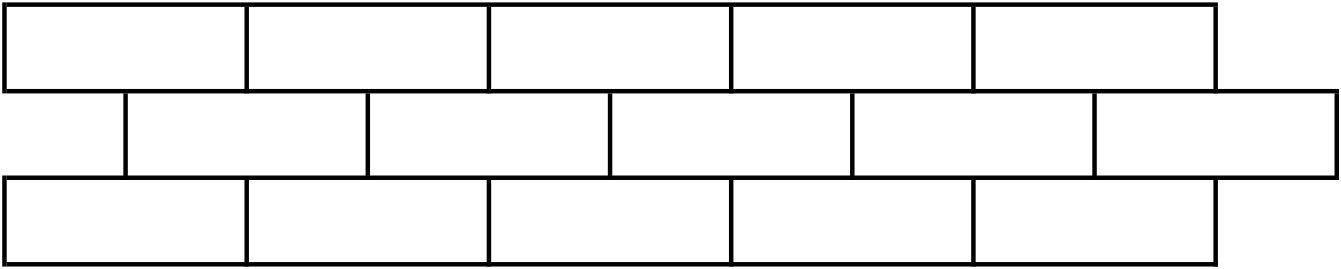
\includegraphics[width=8cm]{brick3x5}
	\end{figure}
	(b) Đếm số cách chọn ra 4 viên gạch, mỗi viên từ 1 hàng trong $4\times5$ viên gạch xếp xen kẽ, sao cho không có 2 viên gạch nào được lấy ra nằm kề nhau.
	\begin{figure}[H]
		\centering
		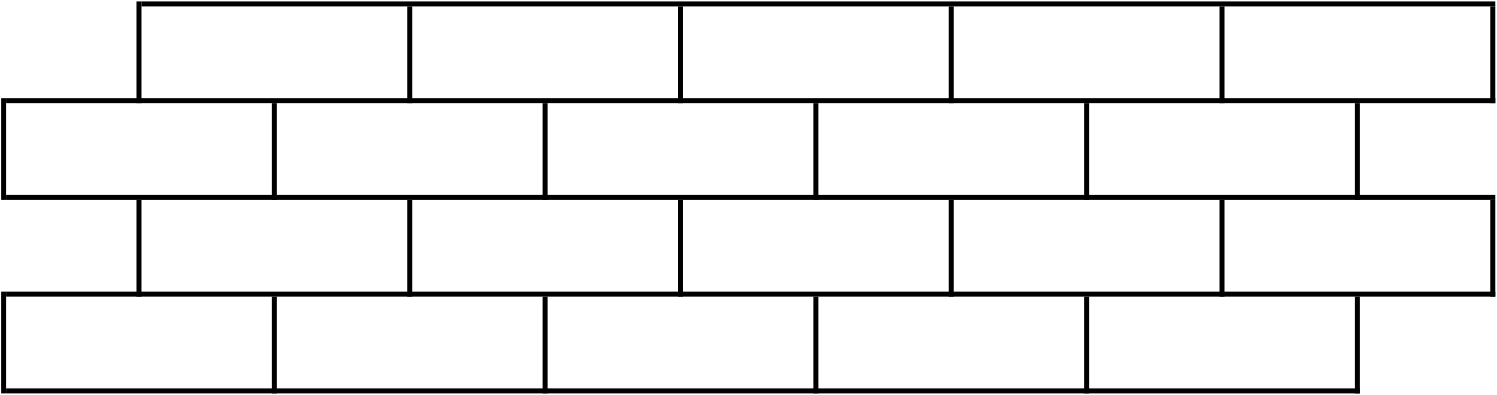
\includegraphics[width=8cm]{brick4x5}
	\end{figure}
	(c) Cho $m,n\in\mathbb{N}^\star$. Đếm số cách chọn ra $m$ viên gạch, mỗi viên từ 1 hàng trong $m\times n$ viên gạch xếp xen kẽ, sao cho không có 2 viên gạch nào được lấy ra nằm kề nhau. (d) Cho $m,n,k\in\mathbb{N}^\star$. Đếm số cách chọn ra $k$ viên gạch, không nhất thiết mỗi viên từ 1 hàng trong $m\times n$ viên gạch xếp xen kẽ, sao cho không có 2 viên gạch nào được lấy ra nằm kề nhau. (e${}^\star$) Mở rộng cho trường hợp $m\times n$ với số gạch mỗi hàng có thể khác nhau, cụ thể là hàng $i$ chứa $a_i\in\mathbb{N}^\star$ viên gạch, $\forall i = 1,\ldots,m$ với 2 trường hợp: (i) Mỗi viên từ 1 hàng. (ii) Lấy $k\in\mathbb{N}^\star$ viên gạch, mỗi hàng có thể lấy nhiều viên.
\end{baitoan}

\begin{nhanxet}[Left-right symmetry -- Đối xứng trái phải]
	Nếu số viên gạch của mỗi hàng bằng nhau \& được sắp xen kẽ như (a) \& (b), thì thứ tự viên gạch đầu tiên từ bên trái của mỗi hàng lồi ra hay thụt vào không quan trọng, vì có thể lấy đối xứng gương trái--phải để chuyển đổi 2 trường hợp đó. Cũng chú ý đến tính đối xứng trên--dưới (top-bottom symmetry).
\end{nhanxet}

\begin{proof}
	Số cách chọn gạch từ 3 hàng, mỗi hàng $n$ viên gạch: $(n - 1)(n - 2)^2 + (n - 1)^2 = (n - 1)(n^2 - 3n + 3)$, $\forall n\in\mathbb{N}^\star$, $n\ge2$. Số cách chọn gạch từ 4 hàng, mỗi hàng $n\in\mathbb{N}^\star$ viên gạch: $(n^2 - 3n + 3)^2$, $\forall n\in\mathbb{N}^\star$, $n\ge2$.
\end{proof}

\begin{itemize}
	\item C++ codes:
	\begin{itemize}
		\item (DKAK): \url{https://github.com/NQBH/advanced_STEM_beyond/blob/main/VMC/C++/brick_DPAK.cpp}.
		\item (NLDK): \url{https://github.com/NQBH/advanced_STEM_beyond/blob/main/VMC/C++/brick_NLDK.cpp}.
	\end{itemize}
\end{itemize}

%------------------------------------------------------------------------------%

\section{Nhị thức Newton \& đa thức}

\begin{theorem}[Binomial theorem]
	(i) $(a + b)^n = \sum_{i=0}^n C_n^ia^{n-i}b^i$, $\forall a,b\in\mathbb{R}$, $\forall n\in\mathbb{N}$. (ii) $\sum_{i=0}^n C_n^i = 2^n$. (iii)
	\begin{equation*}
		\sum_{i=0}^n (-1)^iC_n^i = 0\Leftrightarrow\sum_{i=0,i:{\rm even}}^n C_n^i = \sum_{i=0,i:{\rm odd}}^n C_n^i\Leftrightarrow\left\{\begin{split}
			C_{2n}^0 + C_{2n}^2 + \cdots + C_{2n}^{2n} &= C_{2n}^1 + C_{2n}^3 + \cdots + C_{2n}^{2n-1},\\
			C_{2n+1}^0 + C_{2n+1}^2 + \cdots + C_{2n+1}^{2n} &= C_{2n+1}^1 + C_{2n+1}^3 + \cdots + C_{2n+1}^{2n+1}.
		\end{split}\right.
	\end{equation*}	
\end{theorem}

\begin{baitoan}
	Khai triển: (a) $(a + b + c)^n$, $\forall a,b,c\in\mathbb{R}$, $\forall n\in\mathbb{N}^\star$. (b) $(a + b + c + d)^n$, $\forall a,b,c,d\in\mathbb{R}$, $\forall n\in\mathbb{N}^\star$. (c) $\left(\sum_{i=1}^m a_i\right)^n$, $\forall m,n\in\mathbb{N}^\star$, $\forall a_i\in\mathbb{R}$, $\forall i = 1,\ldots,m$. (d) $z^n$, $\forall z\in\mathbb{C}$, $\forall n\in\mathbb{N}^\star$ với $z = a + bi$, $a\coloneqq\Re z$, $b\coloneqq\Im z$.
\end{baitoan}

%------------------------------------------------------------------------------%

\subsection{Combinatorial identities -- Đẳng thức tổ hợp}
Các phương pháp chứng minh đẳng thức tổ hợp:
\begin{itemize}
	\item Sử dụng phương pháp quy nạp toán học.
	\item Bắt đầu từ 1 đẳng thức tổ hợp, e.g., 1 khai triển của 1 biểu thức, sau đó lấy đạo hàm 2 vế (có thể lấy đạo hàm nhiều lần nếu cần thiết).
	\item Bắt đầu từ 1 đẳng thức tổ hợp, e.g., 1 khai triển của 1 biểu thức, sau đó lấy tích phân 2 vế (có thể lấy tích phân bội nếu cần thiết).
	\item Lý luận tổ hợp: Đếm bằng 2 cách.
\end{itemize}

%------------------------------------------------------------------------------%

\subsubsection{Pascal's rule -- Quy tắc Pascal}
In mathematics, {\it Pascal's rule} (or {\it Pascal's formula}) is a combinatorial identity about \href{https://en.wikipedia.org/wiki/Binomial_coefficient}{binomial coefficients}. The binomial coefficients are the numbers that appear in \href{https://en.wikipedia.org/wiki/Pascal%27s_triangle}{Pascal's triangle}.

\begin{theorem}[Pascal's rule]
	One has
	\begin{equation}
		\label{Pascal's rule}
		\tag{Pasr}
		C_{n-1}^k + C_{n-1}^{k-1} = C_n^k,\mbox{ i.e., }\binom{n - 1}{k} + \binom{n - 1}{k - 1} = \binom{n}{k},\ \forall n,k\in\mathbb{N}^\star,
	\end{equation}
	where $\binom{n}{k}$ is the binomial coefficient, namely the coefficient of the $x^k$ term in the \href{https://en.wikipedia.org/wiki/Polynomial_expansion}{expansion} of $(1 + x)^n$. There is no restriction on the relative sizes of $n,k$; in particular, \eqref{Pascal's rule} remains valid when $n < k$ since $\binom{n}{k} = 0$ whenever $n < k$.
\end{theorem}
Together with the boundary conditions $\binom{n}{0} = \binom{n}{n} = 1$, $\forall n\in\mathbb{N}$, Pascal's rule determines that
\begin{equation*}
	\binom{n}{k} = \frac{n!}{k!(n - k)!},\ \forall n,k\in\mathbb{N},\,0\le k\le n.
\end{equation*}
In this sense, Pascal's rule is the \href{https://en.wikipedia.org/wiki/Recurrence_relation}{recurrence relation} that defines the binomial coefficients.

\begin{problem}
	Prove Pascal's rule \eqref{Pascal's rule}.
\end{problem}
For a combinatorial- \& an algebraic proofs of Pascal's rule, see, e.g., \href{https://en.wikipedia.org/wiki/Pascal%27s_rule}{Wikipedia{\tt/}Pascal's rule}.

\begin{proof}[A combinatorial proof of Pascal's rule when $n\in\mathbb{N}^\star$]
	$\binom{n}{k}$ equals the number of subsets with $k$ elements from a set with $n$ elements. Suppose 1 particular element is uniquely labeled $X$ in a set with $n$ elements. To construct a subset of $k$ elements containing $X$, include $X$ \& choose $k - 1$ elements from the remaining $n - 1$ elements in the set. There are $\binom{n - 1}{k - 1}$ such subsets. To construct a subset of $k$ elements not containing $X$, choose $k$ elements from the remaining $n - 1$ elements in the set. There are $\binom{n - 1}{k}$ such subsets. Every subset of $k$ elements either contains $X$ or not. The total number of subsets with $k$ elements in a set of $n$ elements is the sum of the number of subsets containing $X$ \& the number of subsets that do not contain $X$, $\binom{n - 1}{k - 1} + \binom{n - 1}{k}$. This equals $\binom{n}{k}$, hence \eqref{Pascal's rule} holds.
\end{proof}

\begin{proof}[1st algebraic proof of Pascal's rule when $n\in\mathbb{N}^\star$]
	\begin{align*}
		\binom{n - 1}{k} + \binom{n - 1}{k - 1} &= \frac{(n - 1)!}{k!(n - 1 - k)!} + \frac{(n - 1)!}{(k - 1)!(n - k)!} = (n - 1)!\left(\frac{1}{k!(n - 1 - k)!} + \frac{1}{(k - 1)!(n - k)!}\right)\\
		&= (n - 1)!\left(\frac{n - k}{k!(n - k)!} + \frac{k}{n!(n - k)!}\right) = (n - 1)!\frac{n}{k!(n - k)!} = \frac{n!}{k!(n - k)!} = \binom{n}{k}.
	\end{align*}
\end{proof}

\begin{proof}[2nd algebraic proof of Pascal's rule when $n\in\mathbb{C}$]
	An alternative algebraic proof using the alternative definition of binomial coefficients $\binom{n}{k} = \frac{n(n - 1)\cdots(n - k + 1)}{k!}$, which is used as the extended definition of the binomial coefficient when $n\in\mathbb{C}$, hence \eqref{Pascal's rule} holds more generally for $n\in\mathbb{C}$.
\end{proof}
Pascal's rule can be generalized to \href{https://en.wikipedia.org/wiki/Multinomial_coefficient}{multinomial coefficients}.

\begin{theorem}[Generalized Pascal's rule]
	For any $p\in\mathbb{N}$, $p\ge2$, $k_1,\ldots,k_p\in\mathbb{N}$, $n = \sum_{i=1}^p k_i\ge1$,
	\begin{equation}
		\label{generalized Pascal's rule}
		\tag{gPasr}
		\binom{n - 1}{k_1 - 1,k_2,k_3,\ldots,k_p} + \binom{n - 1}{k_1,k_2 - 1,k_3,\ldots,k_p} + \cdots + \binom{n - 1}{k_1,k_2,k_3,\ldots,k_p - 1} = \binom{n - 1}{k_1,k_2,k_3,\ldots,k_p},
	\end{equation}
	where $\binom{n}{k_1,k_2,\ldots,k_p}$ is the coefficient of the $\prod_{i=1}^p x_i^{k_i}$ term in the expansion of $\left(\sum_{i=1}^p x_i\right)^n$.
\end{theorem}

\begin{problem}
	Prove generalized Pascal's rule \eqref{generalized Pascal's rule} in both combinatorial \& algebraic ways.
\end{problem}

%------------------------------------------------------------------------------%

\begin{baitoan}[\cite{Phuong_to_hop}, VD2, p. 54]
	Chứng minh $\sum_{i=1}^n iC_n^i = n2^{n-1}$, $\forall n\in\mathbb{N}^\star$ bằng 4 cách: (a) Sử dụng phương pháp quy nạp toán học. (b) Biến đổi số hạng tổng quát nhờ đẳng thức Pascal. (c) Xét khai triển $(1 + x)^n$ rồi lấy đạo hàm 2 vế. (d) Lý luận tổ hợp.
\end{baitoan}

\begin{baitoan}[\cite{Phuong_to_hop}, VD3, p. 54]
	Chứng minh $\sum_{i=0}^n \dfrac{C_n^i}{i+1} = \dfrac{2^{n+1} - 1}{n + 1}$, $\forall n\in\mathbb{N}^\star$ bằng 4 cách: (a) Sử dụng phương pháp quy nạp toán học. (b) Biến đổi số hạng tổng quát nhờ đẳng thức Pascal. (c) Xét khai triển $(1 + x)^n$ rồi lấy tích phân $\int_0^1$ 2 vế. (d) Lý luận tổ hợp.
\end{baitoan}

\begin{baitoan}[\cite{Phuong_to_hop}, VD4, p. 55]
	Chứng minh $\sum_{i=0}^n (C_n^i)^2 = C_{2n}^n$, $\forall n\in\mathbb{N}^\star$ bằng 2 cách: (a) Tính hệ số của $x^n$ trong khai triển của nhị thức Newton của $(x + 1)^{2n} = (x + 1)^n(1 + x)^n$ bằng 2 cách. (d) Lý luận tổ hợp.
\end{baitoan}

\begin{baitoan}[\cite{Phuong_to_hop}, VD5, p. 55, ĐH-A 2006]
	(a) Tìm hệ số của số hạng chứa $x^{26}$ trong khai triển nhị thức Newton của $\left(\dfrac{1}{x^4} + x^7\right)^n$ biết $\sum_{i=1}^n C_{2n+1}^i = 2^{20} - 1$. (b) Tìm hệ số của số hạng chứa $x^k$ trong khai triển nhị thức Newton của $\left(x^a + x^n\right)^n$ biết $\sum_{i=1}N C_{2n+1}^i = 2^{n_0} - 1$ với $n_0\in\mathbb{N}^\star$, $a,b\in\mathbb{R}$.
\end{baitoan}



%------------------------------------------------------------------------------%

\section{Phân vùng số nguyên \& nguyên tắc loại suy}

%------------------------------------------------------------------------------%

\section{Generating function -- Hàm sinh}
{\bf Idea of generating functions.} If we want to find a formula for some function $f(n)$ with $n\in\mathbb{N}$, then we can form the generating function of $f(n)$:
\begin{equation}
	\label{generating function}
	\tag{genf}
	F(x)\coloneqq\sum_{n\ge0} f(n)x^n = f(0) + f(1)x + f(2)x^2 + \cdots + f(n)x^n + \cdots,
\end{equation}
so that $a_n$ is the coefficient of $x^n$ in the Taylor series expansion of $F(x)$ defined by \eqref{generating function}.

Here we are concerned with formal power series, \& questions of convergence do not come up (at least for elementary applications). Sometimes this power series has a nice closed form \& then we can manipulate this function \& get information about $f(n)$, $\forall n\in\mathbb{N}$.

-- Ở đây chúng ta quan tâm đến chuỗi lũy thừa chính thức, \& các câu hỏi về sự hội tụ không xuất hiện (ít nhất là đối với các ứng dụng cơ bản). Đôi khi chuỗi lũy thừa này có dạng đóng đẹp \& sau đó chúng ta có thể thao tác hàm này \& lấy thông tin về $f(n)$, $\forall n\in\mathbb{N}$.

\begin{dinhly}[Some basic properties of generating function -- Vài tính chất cơ bản của hàm sinh]
	Cho $G(a,x),G(b,x)$ là hàm sinh tương ứng của 2 dãy số $a= \{a_n\}_{n=0}^\infty,b = \{b_n\}_{n=0}^\infty$.
	\item(i) Nếu tồn tại $k\in\mathbb{N}$ mà $a_i = 0$, $\forall i\in\mathbb{N}$, $i < k$, \& $b_n = a_{n+k}$, $\forall n\in\mathbb{N}$, thì $G(a,x) = x^kG(b,x)$.
	\item(ii) Nếu $b_n = \sum_{i=0}^n a_i$, $n\in\mathbb{N}$, thì $G(b,x) = \dfrac{G(a,x)}{1 - x}$.
\end{dinhly}

\begin{dinhnghia}[Generalized binomial coefficient -- Hệ số nhị thức mở rộng]
	Với $x\in\mathbb{R},k\in\mathbb{N}$, {\rm hệ số nhị thức mở rộng} $\binom{x}{k}$ được định nghĩa bởi
	\begin{equation*}
		\binom{x}{k}\coloneqq\left\{\begin{split}
			&\frac{x(x - 1)\cdots(x - k + 1)}{k!}&&\mbox{if } k\in\mathbb{N}^\star,\\
			&1&&\mbox{if } k = 0.
		\end{split}\right.
	\end{equation*}	
\end{dinhnghia}



\begin{problem}[\cite{Shahriari2022}, p. 4]
	Let $\{a_n\}_{n=0}^\infty$ be a sequence defined by
	\begin{equation*}
		a_0 = 1,\ \sum_{i=0}^n a_ia_{n-i} = 1,\ \forall n\in\mathbb{N}^\star.
	\end{equation*}
	(a) Let $F(x)\coloneqq\sum_{i=0}^\infty a_ix^i = a_0 + a_1x + a_2x^2 + \cdots$ be the generating function of $\{a_n\}_{n=0}^\infty$. Prove: $F(x)F(x) = \dfrac{1}{1 - x}$, thus $F(x) = \dfrac{1}{\sqrt{1 - x}}$. (b) Prove: $a_n = \dfrac{(2n - 1)!!}{2^nn!} = \dfrac{1\cdot3\cdot5\cdot(2n - 1)}{2^nn!}$, $\forall n\in\mathbb{N}^\star$.
\end{problem}

\begin{baitoan}
	(a) Đếm số cách chọn ra $15$ \$ từ $20$ người nếu $19$ người đầu, mỗi người có thể đưa ra nhiều nhất $1$ \$, người thứ $20$ có thể đưa ra $1$ \$, $5$ \$, hoặc không \$ nào. (b) Đếm số cách chọn ra $m\in\mathbb{N}^\star$ \$ từ $n\in\mathbb{N}^\star$ người nếu $k\in\mathbb{N}$ người đầu, mỗi người có thể đưa ra nhiều nhất $a$ \$, $n - k\in\mathbb{N}$ người sau có thể đưa ra $b_1,b_2,\ldots$, hoặc $b_l$ \$ với $b_i\in\mathbb{N}$, $\forall i\in[l]$, $b_i\ne b_j$, $\forall i,j\in[l]$, $i\ne j$.
\end{baitoan}

\begin{baitoan}
	Dùng hàm sinh, giải phương trình nghiệm nguyên
	\begin{equation*}
		\sum_{i=1}^m x_i = n\mbox{ s.t. } m_i\le x_i\le M_i\mbox{ where } m_i,M_i\in\mathbb{Z},\ m_i\le M_i,\ \forall i\in[m].
	\end{equation*}
\end{baitoan}

%------------------------------------------------------------------------------%

\section{Graph Theory -- Lý Thuyết Đồ Thị}
\textbf{\textsf{Resources -- Tài nguyên.}}
\begin{enumerate}
	\item \cite{Andreescu_Dospinescu2010}. {\sc Titu Andreescu, Gabriel Dospinescu}. {\it Problems From the Book}. Chap. 6: {\it Some Classical Problems in Extremal Graph Theory -- Vài Bài Toán Cổ Điển trong Lý Thuyết Đồ Thị Cực Trị}, pp. 119--136.
	
	\item \cite{Valiente2002, Valiente2021}. {\sc Gabriel Valiente}. {\it Algorithms on Trees \& Graphs With Python Code}. 2e.
\end{enumerate}
``In mathematics \& computer science, {\it graph theory} is the study of \href{https://en.wikipedia.org/wiki/Graph_(discrete_mathematics)}{\it graphs}, which are \href{https://en.wikipedia.org/wiki/Mathematical_structures}{mathematical structures} used to model pairwise relations between objects. A graph in this context is made up of \href{https://en.wikipedia.org/wiki/Vertex_(graph_theory)}{\it vertices} (also called {\it nodes} or {\it points}) which are connected by \href{https://en.wikipedia.org/wiki/Glossary_of_graph_theory_terms#edge}{\it edges} (also called {\it arcs, links} or {\it lines}). A distinction is made between {\it undirected graphs}, where edges link 2 vertices symmetrically, \& {\it directed graphs}, where edges link 2 vertices asymmetrically. Graphs are 1 of the principal objects of study in \href{https://en.wikipedia.org/wiki/Discrete_mathematics}{discrete mathematics}.'' -- \href{https://en.wikipedia.org/wiki/Graph_theory}{Wikipedia{\tt/}graph theory}.

Graphs are such a good way of organizing certain kinds of information \& formulating problems in discrete mathematics in general \& combinatorics \& related fields of mathematics in particular. Intuitively, a graph is a set of dots -- called {\it vertices} -- where some of the dots are connected to some of the other dots. The connections are called {\it edges}. Each edge of a graph connects just 2 vertices \& so it can be represented as a pair of vertices.

-- Đồ thị là 1 cách rất hay để sắp xếp một số loại thông tin \& xây dựng các bài toán trong toán học rời rạc nói chung \& tổ hợp \& các lĩnh vực toán học liên quan nói riêng. Theo trực giác, đồ thị là một tập hợp các chấm -- được gọi là các {\it đỉnh} -- trong đó một số chấm được kết nối với một số chấm khác. Các kết nối được gọi là các {\it cạnh}. Mỗi cạnh của đồ thị chỉ kết nối 2 đỉnh \& do đó nó có thể được biểu diễn dưới dạng một cặp đỉnh.

``Đồ thị là 1 mô hình toán học diễn tả 1 cách rất tường minh những mối quan hệ 2 ngôi (1 chiều cũng như 2 chiều) giữa các đối tượng cần được xem xét. Chính vì vậy, đồ thị được sử dụng rộng rãi trong rất nhiều lĩnh vực khác nhau; e.g., khoa học, kỹ thuật, kinh tế, xã hội, etc.'' -- \cite[Sect. 0.1.5, p. 13]{Thanh_computational_complexity_theory}

\subsection{Trees \& graphs: Some basic concepts -- Cây \& đồ thị: Vài khái niệm cơ bản}
Definitions in graph theory vary. For a comprehensive list of concepts in graph theory, see, e.g., \href{https://en.wikipedia.org/wiki/Glossary_of_graph_theory}{Wikipedia{\tt/}glossary of graph theory}. A graph consists of a set of vertices and
a set of edges. Intuitively (and visually), an edge is a direct connection between two vertices. More formally, an edge is a set consisting of
a pair of vertices.

The notion of graph which is most useful in computer science is that of a directed graph or just a graph. A graph is a combinatorial structure consisting of a finite nonempty set of objects, called vertices, together with a finite (possibly empty) set of ordered pairs of vertices, called directed edges or arcs.

-- Khái niệm đồ thị hữu ích nhất trong khoa học máy tính là đồ thị có hướng hoặc chỉ là đồ thị. Đồ thị là 1 cấu trúc tổ hợp bao gồm 1 tập hợp hữu hạn không rỗng các đối tượng, được gọi là các đỉnh, cùng với 1 tập hợp hữu hạn (có thể rỗng) các cặp đỉnh có thứ tự, được gọi là các cạnh có hướng hoặc cung.

\begin{definition}[Graphs \& subgraphs, \cite{Shahriari2022}, Def. 2.17, p. 54]
	A {\rm simple graph} (or just a {\rm graph}) $G$ is a pair of sets $(V,E)$ where $V$ is a nonempty set called the set of {\rm vertices} of $G$, \& $E$ is a (possibly empty) set of unordered pairs of distinct elements of $V$. The set $E$ is called the set of {\rm edges} of $G$. If the number of vertices of $G$ is finite, then $G$ is a {\rm finite graph} (or a {\rm finite simple graph}).
	
	If $G = (V,E)$ \& $H = (V',E')$ are both graphs, then $H$ is a {\rm subgraph} of $G$ if $V'\subseteq V$ \& $E'\subseteq E$.
\end{definition}

\begin{baitoan}
	Vẽ đồ thị Peterson $G_{\rm Peterson} = (V,E)$ \& mô tả cụ thể $V,E$.
\end{baitoan}
To construct a subgraph of a graph given, we take some of the vertices \& some of the edges, but we have to make sure that we have included all the vertices of the edges that we chose.

\begin{definition}[Directed graph, \cite{Valiente2021}, Def. 1.1, p. 3]
	A {\rm graph} $G = (V,E)$ consists of a finite nonempty set $V$ of vertices \& a finite set $E\subseteq V\times V$ of edges. The {\rm order} of a graph $G = (V,E)$, denoted by $n$, is the number of vertices, $n = |V|$ \& the {\rm size}, denoted by $m$, is the number of edges, $m = |E|$. An edge $e = (v,w)$ is said to be {\rm incident} with vertices $v$ \& $w$, where $v$ is the {\rm source} \& $w$ the {\rm target} of edge $e$, \& vertices $v,w$ are said to be {\rm adjacent}. Edges $(u,v),(v,w)$ are said to be {\rm adjacent}, as are edges $(u,v),(w,v)$, \& also edges $(v,u),(v,w)$.
\end{definition}

\begin{dinhnghia}[Đồ thị có hướng]
	1 {\rm đồ thị} $G = (V,E)$ bao gồm 1 tập hữu hạn không rỗng $V$ các đỉnh \& 1 tập hữu hạn $E\subseteq V\times V$ các cạnh. {\rm Bậc} của 1 đồ thị $G = (V,E)$, ký hiệu là $n$, là số đỉnh, $n = |V|$ \& {\rm size}, ký hiệu là $m$, là số cạnh, $m = |E|$. Một cạnh $e = (v,w)$ được gọi là {\rm incident} với các đỉnh $v$ \& $w$, trong đó $v$ là {\rm source} \& $w$ {\rm target} của cạnh $e$, \& các đỉnh $v,w$ được gọi là {\rm kề}. Các cạnh $(u,v),(v,w)$ được gọi là {\rm kề}, cũng như các cạnh $(u,v),(w,v)$, \& cũng vậy các cạnh $(v,u),(v,w)$.
\end{dinhnghia}
Graphs are often drawn as a set of points in the plane \& a set of arrows, each of which joins 2 (not necessarily different) points. In a drawing of a graph $G = (V,E)$, each vertex $v\in V$ is drawn as a point or a small circle \& each edge $(v,w)\in E$ is drawn as an arrow from point or circle of vertex $v$ to the point or circle corresponding to vertex $w$.

-- Đồ thị thường được vẽ như một tập hợp các điểm trên mặt phẳng \& một tập hợp các mũi tên, mỗi mũi tên nối 2 điểm (không nhất thiết phải khác nhau). Trong bản vẽ đồ thị $G = (V,E)$, mỗi đỉnh $v\in V$ được vẽ như một điểm hoặc một đường tròn nhỏ \& mỗi cạnh $(v,w)\in E$ được vẽ như một mũi tên từ điểm hoặc đường tròn của đỉnh $v$ đến điểm hoặc đường tròn tương ứng với đỉnh $w$.

A vertex has 2 degrees in a graph, one given by the number of edges coming into the vertex \& the other given by the number of edges in the graph going out of the vertex.

-- Mỗi đỉnh có 2 bậc trong đồ thị, một bậc được xác định bởi số cạnh đi vào đỉnh \& bậc còn lại được xác định bởi số cạnh trong đồ thị đi ra khỏi đỉnh.

\begin{definition}[\cite{Valiente2021}, Def. 1.2, p. 4]
	The {\rm indegree} of a vertex $v$ in a graph $G = (V,E)$ is the number of edges in $G$ whose target is $v$, i.e., ${\rm indeg}(v) = |\{(u,v)|(u,v)\in E\}|$. The {\rm outdegree} of a vertex $v$ in a graph $G = (V,E)$ is the number of edges in $G$ whose source is $v$, i.e., ${\rm outdeg}(v) = |\{(v,w)|(v,w)\in E\}|$. The {\rm degree} of a vertex $v$ in a graph $G = (V,E)$ is the sum of the indegree \& the outdegree of the vertext, i.e., ${\rm deg}(v) = {\rm indeg}(v) + {\rm outdeg}(v)$.
\end{definition}
A basic relationship between the size of a graph \& the degree of its vertices, which will prove to be very useful in analyzing the computational complexity of algorithms on graphs:

-- Mối quan hệ cơ bản giữa kích thước của đồ thị \& bậc của các đỉnh, sẽ rất hữu ích trong việc phân tích độ phức tạp tính toán của các thuật toán trên đồ thị:

\begin{theorem}
	Let $G = (V,E)$ be a graph with $n$ vertices \& $m$ edges, \& let $V = \{v_1,\ldots,v_n\}$. Then
	\begin{equation*}
		\sum_{i=1}^n {\rm indeg}(v_i) = \sum_{i=1}^n {\rm outdeg}(v_i) = m.
	\end{equation*}
\end{theorem}

\begin{definition}[Multigraphs, general graphs, \cite{Shahriari2022}, Def. 2.20, p. 54]
	In the definition of a graph, if we allow $E$ to be a multiset -- i.e., allow {\rm repeated edges} -- then $G$ is called a {\rm multigraph} or a {\rm graph with repeated edges}. If we also allow pairs of non-distinct elements in $E$ -- i.e., allow {\rm loops} -- then $G$ is called a {\rm general graph} or a {\rm graph with repeated edges \& loops}.
\end{definition}

\begin{dinhnghia}[Đa đồ thị, đồ thị tổng quát]
	Trong định nghĩa của đồ thị, nếu chúng ta cho phép $E$ là một đa tập -- tức là cho phép {\rm các cạnh lặp lại} -- thì $G$ được gọi là {\rm đa đồ thị} hoặc {\rm đồ thị có các cạnh lặp lại}. Nếu chúng ta cũng cho phép các cặp phần tử không phân biệt trong $E$ -- tức là cho phép {\rm các vòng lặp} -- thì $G$ được gọi là {\rm đồ thị tổng quát} hoặc {\rm đồ thị có các cạnh lặp lại \& vòng lặp}.
\end{dinhnghia}
If a graph $G$ does not have any double edges or loops then $G$is a simple graph. If a graph $G$ has repeated edges but no loops, then $G$ is a multigraph. If $G$ has both repeated edges \& repeated loops, then $G$ would be a general graph.

\begin{remark}[\cite{Shahriari2022}, Rmk. 2.22, p. 55]
	If $G = (V,E)$ is a general graph \& $e\in E$ is an edge of $G$, then, unlike in the case of simple graphs, we cannot necessarily identify $e$ by its vertices. I.e., it will be inadequate to say $e = \{v,w\}$, where $v,w\in V$. This is because there may be multiple edges connecting $v$ \& $w$. Hence, to be formally correct, we should say that a general graph consists of 2 sets $V$ \& $E$ \& an incidence map that gives 2 vertices for each $e\in E$. I.e., every edge will have its own name in addition to being associated with its 2 vertices. To avoid unnecessary clutter, in what follows we will continue to identify edges of general graphs as pairs of vertices unless there is a need to be more formal.
	
	-- Nếu $G = (V,E)$ là một đồ thị tổng quát \& $e\in E$ là một cạnh của $G$, thì, không giống như trong trường hợp của đồ thị đơn giản, chúng ta không nhất thiết phải xác định $e$ theo các đỉnh của nó. Tức là, sẽ không đủ nếu nói $e = \{v,w\}$, trong đó $v,w\in V$. Điều này là do có thể có nhiều cạnh kết nối $v$ \& $w$. Do đó, để chính xác về mặt hình thức, chúng ta phải nói rằng một đồ thị tổng quát bao gồm 2 tập hợp $V$ \& $E$ \& một bản đồ tới cung cấp 2 đỉnh cho mỗi $e\in E$. Tức là, mỗi cạnh sẽ có tên riêng của nó ngoài việc được liên kết với 2 đỉnh của nó. Để tránh sự lộn xộn không cần thiết, trong phần sau, chúng ta sẽ tiếp tục xác định các cạnh của đồ thị tổng quát là các cặp đỉnh trừ khi cần phải chính thức hơn.
\end{remark}

\begin{definition}[Order, adjacency, incidence, \cite{Shahriari2022}, Def. 2.23, p. 55]
	Let $G = (V,E)$ be a general graph. Then $|V|$, the number of vertices, is called the {\rm order} of $G$. If $\alpha = \{x,y\}\in E$ -- i.e., $\alpha$ is an edge connecting the vertices $x,y$ -- then we say that $x$ \& $y$ are {\rm vertices} or {\rm ends} of $\alpha$, that $\alpha$ {\rm joints} $x$ \& $y$, that $x$ \& $y$ are {\rm adjacent}, \& that $x$ \& $\alpha$ are {\rm incident}.
\end{definition}

\begin{definition}[Degree of a vertex, \cite{Shahriari2022}, Def. 2.24, p. 55]
	If $x$ is a vertex of a graph $G$, then the number of edges incident with $x$ is called the {\rm degree} (or the {\rm valence}) of $x$. In the case of general graphs, a loop at a vertex $x$ contributes $2$ to the degree of $x$.
\end{definition}
The degree of a vertex is the number of edges incident with it \& note that, in a general graph, a loop contributes 2 to the degree of its vertex. One usually records the degrees of each vertices of a graph in a table.

-- Bậc của một đỉnh là số cạnh liên quan đến nó \& lưu ý rằng, trong một đồ thị tổng quát, một vòng lặp đóng góp 2 vào bậc của đỉnh của nó. Người ta thường ghi lại bậc của mỗi đỉnh của đồ thị trong một bảng.

Roughly speaking, in graph theory, we are not concerned with the labels of the vertices. So, if we keep the vertices \& edges intact, but rearrange the names of the vertices, we get a new graph that is basically the same graph as $G$. We say that these 2 graphs are {\it isomorphic}.

-- Nói một cách đại khái, trong lý thuyết đồ thị, chúng ta không quan tâm đến nhãn của các đỉnh. Vì vậy, nếu chúng ta giữ nguyên các đỉnh \& cạnh, nhưng sắp xếp lại tên của các đỉnh, chúng ta sẽ có một đồ thị mới về cơ bản là cùng một đồ thị với $G$. Chúng ta nói rằng 2 đồ thị này là {\it đẳng cấu}.

More technically, in combinatorial graph theory -- as opposed to topological graph theory -- we are not concerned with how a graph is drawn. The drawing is just a representation that helps us ``see'' the vertices \& the edges. All that matters is the number of vertices \& their adjacencies. Hence, we consider 2 graphs the same if, after we appropriately relabel the vertices of 1 of the graphs, the set of edges of the 2 graphs become the same. 2 such graphs are called isomorphic.

\begin{definition}[Graph isomorphism]
	Let $G,H$ be graphs. The graph $G$ is {\rm isomorphic} to the graph $H$ if there exists a 1-1, onto map $f:V(G)\to V(H)$ s.t. $\{x,y\}$ is an edge of $G$ iff $\{f(x),f(y)\}$ is an edge of $H$. Such a map $f$ is called an {\rm  isomorphism} between $G$ \& $H$.
\end{definition}

\begin{example}
	In the Peterson graph, every vertex has degree $3$.
\end{example}
A few oft-used terms to graph vocabularies.

\begin{definition}[Isolated vertex, leaf, \cite{Shahriari2022}, Def. 10.2, p. 362]
	Let $G$ be a graph. A vertex with degree $0$ is called an {\rm isolated vertex}, while a vertex with degree $1$ is called a {\rm leaf}.
\end{definition}

\begin{definition}[Regular graph, \cite{Shahriari2022}, Def. 10.3, p. 362]
	A graph is called {\rm regular of degree $d$} or {\rm$d$-regular} if each vertex has degree equal to $d$.
\end{definition}
In mathematical notation:
\begin{equation*}
	G = (V,E)\mbox{ is a } d\mbox{-regular}\Leftrightarrow\deg v = d,\ \forall v\in V.
\end{equation*}

\begin{definition}[Cubic graph, \cite{Shahriari2022}, Def. 10.4, p. 362]
	A graph is called {\rm cubic} if it is regular of degree $3$ (i.e., if each vertex has degree equal to $3$).
\end{definition}

\subsubsection{Walks, trails, paths, cycles, \& complete graphs}
Walks, trails, \& paths in a graph are alternating sequences of vertices \& edges in the graph s.t. each edge in the sequence is preceded by its source vertex \& followed by its target vertex. Trails are walks having no repeated edges, \& paths are trails having no repeated vertices.

-- Đường đi, đường mòn, \& đường đi trong đồ thị là chuỗi xen kẽ các đỉnh \& cạnh trong đồ thị, tức là mỗi cạnh trong chuỗi được đi trước bởi đỉnh nguồn \& theo sau bởi đỉnh đích. Đường mòn là đường đi không có cạnh lặp lại, \& đường đi là đường mòn không có đỉnh lặp lại.

\begin{definition}[Walk, trail, path, \cite{Valiente2021}, Def. 1.3]
	A {\rm walk} from vertex $v_i$ to vertex $v_j$ in a graph is an alternating sequence $[v_i,e_{i+1},v_{i+1},e_{i+2},\ldots,v_{j-1},e_j,v_j]$ of vertices \& edges in the graph, s.t. $e_k = (v_{k-1},v_k)$ for $k = i + 1,\ldots,j$. A {\rm trail} is a walk with no repeated edges, \& a {\rm path} is a trail with no repeated vertices (except, possibly, the initial \& final vertices). The length of a walk, trail, or path is the number of edges in the sequence.
\end{definition}

\begin{dinhnghia}[Đường đi dạo, đường mòn, đường đi]
	1 {\rm đường đi dạo} từ đỉnh $v_i$ đến đỉnh $v_j$ trong một đồ thị là một chuỗi xen kẽ $[v_i,e_{i+1},v_{i+1},e_{i+2},\ldots,v_{j-1},e_j,v_j]$ các đỉnh \& cạnh trong đồ thị, s.t. $e_k = (v_{k-1},v_k)$ với $k = i + 1,\ldots,j$. Một {\rm đường mòn} là một cuộc đi bộ không có cạnh nào lặp lại, \& một {\rm đường đi} là một cuộc đi bộ không có đỉnh nào lặp lại (ngoại trừ, có thể là, các đỉnh đầu \& cuối). Độ dài của một cuộc đi bộ, trail hoặc path là số cạnh trong chuỗi.	
\end{dinhnghia}
Since an edge in a graph is uniquely determined by its source \& target vertices, a walk, trail, or path can be abbreviated by just enumerating either the vertices $[v_i,v_{i+1},\ldots,v_{j-1},v_j]$ or the edges $[e_{i+1},e_{i+2},\ldots,e_j]$ in the alternating sequence $[v_i,e_{i+1},v_{i+1},e_{i+2},\ldots,v_{j-1},e_j,v_j]$ of vertices \& edges.

-- Vì một cạnh trong đồ thị được xác định duy nhất bởi các đỉnh nguồn \& đích của nó, nên một đường đi, đường mòn hoặc đường dẫn có thể được rút gọn chỉ bằng cách liệt kê các đỉnh $[v_i,v_{i+1},\ldots,v_{j-1},v_j]$ hoặc các cạnh $[e_{i+1},e_{i+2},\ldots,e_j]$ trong chuỗi xen kẽ $[v_i,e_{i+1},v_{i+1},e_{i+2},\ldots,v_{j-1},e_j,v_j]$ các đỉnh \& cạnh.

Walks are closed if their initial \& final vertices coincide. -- Đường đi sẽ khép lại nếu đỉnh đầu \& đỉnh cuối trùng nhau.

\begin{definition}[Cycle, \cite{Valiente2021}, Def. 1.4]
	A walk, trail, or path $[v_i,e_{i+1},v_{i+1},e_{i+2},\ldots,v_{j-1},e_i,v_j]$ is said to be {\rm closed} if $v_i = v_j$. A {\rm cycle} is a closed path of length at least $1$.
\end{definition}
The combinatorial structure of a graph encompasses 2 notions of the substructure. A subgraph of a graph is just a graph whose vertex \& edge sets are contained in the vertex \& edge sets of the given graph, resp. The subgraph of a graph induced by a subset of its vertices has as edges the set of edges in the given graph whose source \& target belong to the subset of vertices.

-- Cấu trúc tổ hợp của một đồ thị bao gồm 2 khái niệm về cấu trúc con. Một đồ thị con của một đồ thị chỉ là một đồ thị có tập đỉnh \& cạnh được chứa trong tập đỉnh \& cạnh của đồ thị đã cho, tương ứng. Đồ thị con của một đồ thị được tạo ra bởi một tập con các đỉnh của nó có các cạnh là tập các cạnh trong đồ thị đã cho có nguồn \& đích thuộc về tập con các đỉnh.

\begin{definition}[Subgraph, \cite{Valiente2021}, Def. 1.5, p. 6]
	Let $G = (V,E)$ be a graph, \& let $W\subseteq V$. A graph $(W,S)$ is a {\rm subgraph} of $G$ if $S\subseteq E$. The subgraph of $G$ {\rm induced} by $W$ is the graph $(W,E\cap W\times W)$.
\end{definition}

\begin{dinhnghia}[Đồ thị con]
	Cho $G = (V,E)$ là một đồ thị, \& cho $W\subseteq V$. Một đồ thị $(W,S)$ là một {\rm đồ thị con} của $G$ nếu $S\subseteq E$. Đồ thị con của $G$ {\rm được tạo ra} bởi $W$ là đồ thị $(W,E\cap W\times W)$.
\end{dinhnghia}
The notion of graph which is most often found in mathematics is that of an undirected graph. Unlike the directed edges or edges of a graph, edges of an undirected graph have no direction association with them \& therefore, no distinction is made between the source \& target vertices of an edge. In a mathematical sense, an undirected graph consists of a set of vertices \& a finite set of undirected edges, where each edge has a set of 1 or 2 vertices associated with it. In the computer science view of undirected graphs, though, an undirected graph is the particular case of a directed graph in which for every edge $(v,w)$ of the graph, the reversed edge $(w,v)$ also belongs to the graph. Undirected graphs are also called {\it bidirected}.

-- Khái niệm đồ thị thường thấy nhất trong toán học là đồ thị vô hướng. Không giống như các cạnh hoặc cạnh có hướng của đồ thị, các cạnh của đồ thị vô hướng không có liên kết hướng nào với chúng \& do đó, không có sự phân biệt nào được tạo ra giữa các đỉnh nguồn \& đích của một cạnh. Theo nghĩa toán học, đồ thị vô hướng bao gồm một tập hợp các đỉnh \& một tập hợp hữu hạn các cạnh vô hướng, trong đó mỗi cạnh có một tập hợp gồm 1 hoặc 2 đỉnh được liên kết với nó. Tuy nhiên, theo quan điểm khoa học máy tính về đồ thị vô hướng, đồ thị vô hướng là trường hợp cụ thể của đồ thị có hướng trong đó đối với mọi cạnh $(v,w)$ của đồ thị, cạnh đảo ngược $(w,v)$ cũng thuộc về đồ thị. Đồ thị vô hướng cũng được gọi là {\it song hướng}.

\begin{definition}[Undirected graph, \cite{Valiente2021}, Def. 1.5, p. 6]
	A graph $G = (V,E)$ is {\rm undirected} if $(v,w)\in E\Rightarrow(w,v)\in E$, $\forall v,w\in V$.
\end{definition}

\begin{dinhnghia}[Đồ thị vô hướng]
	Đồ thị $G = (V,E)$ là {\rm vô hướng} nếu $(v,w)\in E\Rightarrow(w,v)\in E$, $\forall v,w\in V$.
\end{dinhnghia}

\begin{baitoan}[\cite{Shahriari2022}, p. 361]
	A soccer ball is often tiled with $12$ pentagons \& $20$ hexagons. Is there anything special about those numbers? If you tile a soccer ball with pentagons \& hexagons, what are the possibilities for the number of pentagons \& the number of hexagons?
	
	-- 1 quả bóng đá thường được lát bằng $12$ hình ngũ giác \& $20$ hình lục giác. Có điều gì đặc biệt về những con số đó không? Nếu bạn lát một quả bóng đá bằng hình ngũ giác \& hình lục giác, thì khả năng có bao nhiêu hình ngũ giác \& số hình lục giác?
\end{baitoan}

\subsubsection{Graphic sequences}

\begin{problem}[\cite{Shahriari2022}, Warm-Up 10.5, p. 363]
	Is there a simple graph with 4 vertices s.t. the degrees of the vertices are $3,2,1,1$. What if the degrees were $2,2,1,1$?
\end{problem}

\begin{proof}
	
\end{proof}

\begin{definition}[Degree sequence of a graph; graphic sequences, \cite{Shahriari2022}, Def. 10.6, p. 363]
	The {\rm degree sequence} of a graph is the list of the degrees of its vertices in non-increasing order.
	
	A non-increasing sequence of nonnegative integers is called {\rm graphic} if there exists a simple graph whose degree sequence is precisely that sequence.
\end{definition}

\begin{question}
	Given a non-increasing sequence of nonnegative integers, when is the sequence graphic?
	
	-- Với một dãy số nguyên không âm không tăng, khi nào thì dãy số này là dãy đồ họa?
\end{question}

\begin{problem}[\cite{Shahriari2022}, Ques. 10.8, p. 363]
	Which of the following sequences are graphic? (a) $7,5,5,4,3,3,3,3,3,2$. (b) $1,1,1$. (c) $5,5,4,3,3,2,2,1$. (d) $7,5,5,4,3,2,2,0$. (e) $6,6,6,6,4,3,3,0$. (f) $7,6,5,5,4,4,4,2,1$.
\end{problem}

\begin{theorem}[\cite{Shahriari2022}, Thm. 10.9, p. 363]
	\label{thm: Euler}
	Let $G = (V,E)$ be a general graph. Let $\{d_i\}_{i=1}^{|V|}$ be the degrees of the vertices. Then
	\begin{equation*}
		\sum_{i=1}^{|V|} d_i = 2|E|.
	\end{equation*}
	In particular, the number of vertices of $G$ with odd degree is even.
\end{theorem}

\begin{theorem}[Havel--Hakimi algorithm]
	\label{thm: Havel--Hakimi algorithm}
	Consider the following 2 sequences of nonnegative integers. Assume the 1st sequence is in nonincreasing order \& $t_s\ge1$: (a) $s,t_1,\ldots,t_s,d_1,\ldots,d_n$. (b) $t_1 - 1,t_2 - 1,\ldots,t_s - 1,d_1,\ldots,d_n$. Sequence (a) is graphic iff sequence (b) is graphic (after possibly rearranging it to make it non-decreasing).
\end{theorem}
Because of this theorem, if you are given a sequence of nonnegative integers \& want to know if it is graphic or not, you repeatedly use Thm. \ref{thm: Havel--Hakimi algorithm} to reduce your sequence to simpler sequences. If, at any point, the simpler sequence is graphic (or not graphic), then so is the original sequence.

-- Vì định lý này, nếu bạn được cung cấp một chuỗi các số nguyên không âm \& muốn biết nó có đồ họa hay không, bạn sử dụng Thm. \ref{thm: Havel--Hakimi algorithm} nhiều lần để rút gọn chuỗi của bạn thành các chuỗi đơn giản hơn. Nếu, tại bất kỳ thời điểm nào, chuỗi đơn giản hơn là đồ họa (hoặc không đồ họa), thì chuỗi ban đầu cũng vậy.

\begin{problem}[\cite{Shahriari2022}, P10.1.1., p. 367]
	A simple graph $G$ has $9$ edges \& the degree of each vertex is at least $3$. What are the possibilities for the number of vertices? Give an example, for each possibility.
\end{problem}

\begin{problem}[\cite{Shahriari2022}, P10.1.2., p. 367]
	Is $7,7,6,5,4,4,4,3,2$ a graphic sequence?
\end{problem}

\begin{problem}[\cite{Shahriari2022}, P10.1.3., p. 367]
	Is there a simple regular graph of degree $5$ with $8$ vertices? Why?
\end{problem}

\begin{problem}[\cite{Shahriari2022}, P10.1.4., p. 367]
	Is there a simple graph on $8$ vertices where half of the degrees are $5$ \& the other half are $3$?
\end{problem}

\begin{problem}[\cite{Shahriari2022}, P10.1.5., p. 367]
	The sequence $7,5,5,4,3,3,3,3,3,2$ is graphic because it is the degree sequence of the simple graph of \cite[Fig. 10.1]{Shahriari2022}. Apply the Havel--Hakimi algorithm Thm. \ref{thm: Havel--Hakimi algorithm} to construct a graph with this degree sequence. Is the resulting graph isomorphic to the graph of \cite[Fig. 10.1]{Shahriari2022}?
\end{problem}

\begin{problem}[\cite{Shahriari2022}, P10.1.6., p. 367]
	Assume that you applied the Havel--Hakimi algorithm to a given sequence, \&, at the end of the process, you arrived at a graphic sequence. You draw a simple graph corresponding to this final sequence, \& work your way back to construct a simple graph with the original sequence as its degree sequence. As you work your way back, is it the case that, at every step, after adding a new vertex, you add edges between this new vertex \& those existing vertices that have the highest degrees? Either prove that you do or provide an example where you don't.
\end{problem}

\begin{problem}[\cite{Shahriari2022}, P10.1.7., p. 367]
	Assume that you have a sequence $d_1,d_2,d_3,d_4$ (with $d_1\ge d_2\ge d_3\ge d_4\ge0$) that you know is not graphic. You consider the sequence $d_1,d_2,d_3,d_4 + 1,1$. Can this sequence be graphic (after possible rearranging so that it is non-increasing order)? Either prove that it is never graphic or given an example where it becomes graphic.
\end{problem}

\begin{problem}[\cite{Shahriari2022}, P10.1.8., p. 367]
	A sequence is graphic if it is the degree sequence of a {\rm simple} graph. Is there a sequence that is not graphic, \& yet is the degree sequence of a multigraph? Either prove that there are no such sequences or give a specific example.
\end{problem}

\begin{problem}[\cite{Shahriari2022}, P10.1.9., p. 367]
	Can you find a sequence that is {\rm not} the degree sequence of a multigraph, but is the degree sequence of a general graph?
\end{problem}

\begin{problem}[\cite{Shahriari2022}, P10.1.10., p. 367]
	Let $d_1,\ldots,d_n$ be a non-increasing sequence of $n$ nonnegative integers. By Thm. \ref{thm: Euler}, if this sequence is the degree sequence of a general graph, then the sum $\sum_{i=1}^n d_i$ is even. What about the converse?
\end{problem}

\begin{problem}[\cite{Shahriari2022}, P10.1.11., p. 367]
	Find 2 non-isomorphic regular simple graphs of degree $3$ \& order $6$.
\end{problem}

\begin{problem}[\cite{Shahriari2022}, P10.1.12., p. 368]
	Apply the Havel--Hakimi algorithm of Thm. \ref{thm: Havel--Hakimi algorithm} to the sequence $5,4,4,2,2,1$. Is the sequence graphic? Can you use the Havel--Hakimi algorithm to find a general graph with this degree sequence that has exactly 1 loop?
\end{problem}

\begin{problem}[\cite{Shahriari2022}, P10.1.13., p. 368]
	(a) Prove that a sequence $d_1,\ldots,d_p$ is a graphic sequence iff the sequence $p - d_p - 1,\ldots,p - d_1 - 1$ is graphic. (b) Is $9,9,9,9,9,9,9,9,8,8,8$ a graphic sequence?
\end{problem}

\begin{problem}[\cite{Shahriari2022}, P10.1.14., p. 368]
	I have a simple graph with $6$ vertices. The degrees of $5$ of the vertices are $5,4,4,2,2$. What are the possibilities for the degree of the 6th vertex?
\end{problem}

\begin{problem}[\cite{Shahriari2022}, P10.1.15., p. 368]
	Can we have a simple graph where the degree sequence consists of all distinct integers? What about a multigraph?
\end{problem}

\begin{problem}[\cite{Shahriari2022}, P10.1.16., p. 368]
	Let $G$ be a simple graph with $94$ vertices. Assume that all the degrees of the vertices are odd integers. Prove that there are at least $3$ vertices with the same degree.
\end{problem}

\begin{problem}[\cite{Shahriari2022}, P10.1.17., p. 368]
	Assume that $a_1\ge a_2\ge\cdots a_n$ is a graphic sequence. Prove that
	\begin{equation*}
		\sum_{i=1}^k a_i\le k(k - 1) + \sum_{i=k+1}^p \min\{k,a_i\}.
	\end{equation*}
\end{problem}

\begin{remark}
	The Erd\H{o}s--Gallai theorem asserts that this necessary condition, together with the trivial condition that the sum of the degrees be even, gives a sufficient condition for identifying graphic sequences. This theorem can be proved (see [Choudrum1986]) by induction on the sum of the degrees. Given a degree sequence satisfying the condition, you subtract $1$ from the smallest degree \& $1$ from 1 of the other degrees (the smallest index $t$ with $a_t > a_{t-1}$ or, if all the degrees are equal, then from $a_{n-1}$). After (tediously) showing that this new sequence also satisfies the Erd\H{o}s--Gallai condition, you use the inductive hypothesis, \& finish the proof using the result in \cite[Prob. P10.1.18, p. 368]{Shahriari2022}.
\end{remark}

\begin{problem}[\cite{Shahriari2022}, P10.1.18., p. 368]
	Let $p,t\in\mathbb{N}^\star$ with $2\le t < p$. Assume $a_1\ge a_2\ge\cdots\ge a_{t-1} > a_t\ge\cdots\ge a_{p-1} > a_p$ is the degree sequence of a simple graph. Prove that $a_1\ge a_2\ge\cdots\ge a_{t-1}\ge a_t + 1\ge\cdots\ge a_{p-1}\ge a_p + 1$ is also the degree sequence of a simple graph.
\end{problem}

\begin{problem}[\cite{Shahriari2022}, P10.1.19., pp. 368--369, Kapoor, Polimeni, Wall1977]
	Does there exist a simple graph with $48$ vertices where the set of the degrees of the vertices is $\{4,7,47\}$? I.e., we want all the degrees of the vertices to be either $4$, or $7$, or $47$, \& for there to be at least 1 vertex with each of these degrees. More generally, let $S = \{a_1,\ldots,a_k\}$ be any nonempty set of $k$ positive integers with $a_1 < a_2 < \cdots < a_k$. Prove that there exists some simple graph $G$ with $a_k + 1$ vertices, where the set of the degrees of the vertices is precisely $S$. (Note that we are not specifying the degree sequence of graph, just the set of numbers that occur as degrees.) You may find the following steps helpful:
	\begin{itemize}
		\item Step 1: Assume $|S| = 1$, \& $S = \{a_1\}$. Give an example of a simple graph where all the degrees are equal to $a_1$.
		\item Step 2: Construct a simple graph $G$ with $p + q$ vertices as follows. Start with a complete graph $K_p$ \& $q$ isolated vertices. Now add an edge between every isolated vertex \& every vertex of $K_p$. What is the set of degrees of $G$?
		\item Step 3: Assume $|S| = 2$, \& $S = \{a_1,a_2\}$ with $a_1 < a_2$. By a judicious choice of $p,q$ in the previous step, given an example of a simple graph where the set of the degrees is precisely $S$.
		\item Step 4: Let $p,q,r,m\in\mathbb{N}^\star$. Assume that $H$ is a simple graph with $r$ vertices, \& that $S_1 = \{b_1,\ldots,b_m\}$ is the set of the degrees of $H$. Construct a simple graph $G$ with $p + q + r$ vertices as follows. Start with a $K_p$ (complete graph of order $p$), a copy of $H$, \& $q$ isolated vertices. Add an edge between every vertex in $K_p$ \& each of the other vertices. What is the set of degrees of the vertices of $G$?
		\item Step 5: To prove the general statement, induct on $|S|$. Using the inductive hypothesis, start with a graph $H$ with degree set equal to $\{a_2 - a_1,a_3 - a_1,\ldots,a_{k-1} - a_1\}$, \& judiciously choose $p,q$ in Step 4.
	\end{itemize}
\end{problem}

\begin{goal}[Tính khả dĩ của dãy bậc của đồ thị]
	Tìm vài dấu hiệu hoặc vài điều kiện cần \& đủ để có thể quyết định liệu 1 dãy số nguyên dương $(a_i)_{i=1}^n\subset\mathbb{N}$ cho trươc có  thể thể là dãy bậc của đồ thị mà không phải vẽ biểu đồ.
\end{goal}

\begin{dinhnghia}[\cite{Ha_Thanh_to_hop}, Def. 7.6, p. 249, Dãy bậc của đồ thị, chuỗi đồ thị]
	{\rm Chuỗi bậc} của đồ thị là dãy bậc của các đỉnh của nó theo thứ tự không tăng. 1 dãy số nguyên không âm không tăng được gọi là {\rm đồ thị} nếu tồn tại 1 đồ thị có chuỗi bậc chính xác là dãy số nguyên không âm đó.
\end{dinhnghia}

\begin{vidu}[Sequence $1,1,\ldots,1$]
	$1,1,1$ không phải là 1 dãy đồ thị vì không thể xây dựng 1 đồ thị có 3 đỉnh sao cho tất cả 3 bậc là $1$. Nhưng $1,1$ \& $1,1,1,1$, hay nói chung các dãy chỉ toàn số $1$ với độ dài là 1 số chẵn, i.e., $\{1\}_{i=1}^{2n}$, $\forall n\in\mathbb{N}^\star$, là các dãy đồ thị, nhưng bất kỳ dãy chỉ toàn số $1$ với độ dài là 1 số lẻ, i.e., $\{1\}_{i=1}^{2n+1}$, $\forall n\in\mathbb{N}^\star$, thì không phải là 1 dãy đồ thị (why?)
\end{vidu}

\begin{dinhly}[Euler's, \cite{Ha_Thanh_to_hop}, Thm. 7.9, p. 250]
	Cho $G = (V,E)$ là đồ thị tổng quát với $d_1,\ldots,d_{|V|}\in\mathbb{N}$ là bậc của các đỉnh. Khi đó $\sum_{i=1}^{|V|} d_i = d_1 + d_2 + \cdots + d_{|V|} = 2|E|$. Nói riêng, số đỉnh của $G$ có bậc lẻ là số chẵn.
\end{dinhly}
Briefly:
\begin{equation*}
	d_1,\ldots,d_{|V|}\mbox{ are degrees of vertices of a graph } G = (V,E)\Rightarrow\sum_{i=1}^{|V|} d_i = 2|E|\Rightarrow|\{i;d_i\not{\divby}\ 2\}|\divby2.
\end{equation*}
Chú ý chiều ngược lại chưa chắc đúng:
\begin{vidu}
	Dãy số $7,5,5,4,3,2,2,0$ không mâu thuẫn với Định lý \ref{thm: Euler} nhưng nó không phải là đồ thị (why?).
\end{vidu}

\begin{question}
	Có thể suy ra được những hệ quả nào từ đẳng thức $\sum_{i=1}^{|V|} d_i = 2|E|$?
\end{question}

\begin{baitoan}
	Cho $G = (V,E)$ là đồ thị tổng quát với $d_1,\ldots,d_p\in\mathbb{N}$ là bậc của các đỉnh. Chứng minh: Bậc cao nhất $d_{\max}\coloneqq\max_{1\le i\le p} d_i$ thỏa $d_{\max}\ge\dfrac{2|E|}{|V|}$.
\end{baitoan}

\begin{baitoan}
	Viết chương trình {\sf C{\tt/}C++, Python} sử dụng định lý Euler \ref{thm: Euler} \& thuật toán Havel--Hakimi \ref{thm: Havel--Hakimi algorithm} để kiểm tra 1 dãy số nguyên không âm được nhập có phải là 1 graphical sequence hay không.
	\item {\sf Input.} Dòng 1 chứa số bộ test $t\in\mathbb{N}^\star$. Tiếp theo, mỗi bộ test gồm 2 dòng: Dòng 1 chứa $n\coloneqq|V|\in\mathbb{N}^\star$: số đỉnh của đồ thị $G = (V,E)$. Dòng 2 chứa dãy $d_1,\ldots,d_n\in \mathbb{N}$.
	\item {\sf Output.} Xuất ra {\tt1} nếu dãy đó là dãy graphical sequence, {\tt0} nếu dãy đó không phải là dãy graphical sequence, nếu chưa quyết định được thì xuất ra dãy không thể giảm được nữa thu được từ thuật toán Havel--Hakimi \ref{thm: Havel--Hakimi algorithm}.
	\item {\sf Sample.}
	\begin{table}[H]
		\centering
		\begin{tabular}{|l|l|}
			\hline
			\verb|graphical_sequence.inp| & \verb|graphical_sequence.out| \\
			\hline
			3 &  \\
			4 &  \\
			3 2 1 1 & \\
			4 &  \\
			2 2 1 1 &  \\
			10 &  \\
			7 7 6 6 6 5 5 4 3 1 &  \\
			9 &  \\
			7 7 6 5 4 4 4 3 2 &  \\
			10 &  \\
			7 5 5 4 3 3 3 3 3 2 &  \\
			\hline
		\end{tabular}
	\end{table}
\end{baitoan}

\begin{proof}
	\begin{itemize}
		\item Input: \url{https://github.com/NQBH/advanced_STEM_beyond/tree/main/combinatorics/input}.
		\item Output: \url{https://github.com/NQBH/advanced_STEM_beyond/tree/main/combinatorics/output}.
		\item Python code:
		\begin{itemize}
			\item LDL's Havel--Hakimi algorithm Python code: \url{https://github.com/NQBH/advanced_STEM_beyond/blob/main/combinatorics/Python/LDL_Havel_Hakimi_alg.py}.
\begin{verbatim}
def havel_hakimi(sequence):
    while True:
        sequence = [d for d in sequence if d != 0]

        if not sequence:
            return True

        # Sort in non-increasing order
        sequence.sort(reverse=True)
        d = sequence.pop(0)

        if d > len(sequence):
            return False

        # Subtract 1 from the next d elements
        for i in range(d):
            sequence[i] -= 1
            if sequence[i] < 0:
                return False

        print(f"After processing: {sequence}, removed: {d}")

def main():
    t = int(input("Enter number of test cases: "))
    for _ in range(t):
        n = int(input("Enter number of members: "))
        sequence = list(map(int, input(f"Enter {n} degree values: ").split()))
        if havel_hakimi(sequence):
            print("YES")
        else:
            print("NO")

if __name__ == "__main__":
    main()
\end{verbatim}
		\end{itemize}
		\item C++ code:
		\begin{itemize}
			\item VNTA's Havel--Hakimi algorithm Python code: \url{https://github.com/NQBH/advanced_STEM_beyond/blob/main/combinatorics/C++/VNTA_Havel_Hakimi_alg.cpp}.
\begin{verbatim}
#include <bits/stdc++.h>
using namespace std;

void print(vector<int>&d) {
    for (int x : d) cout<<x<<' ';
    cout<<'\n';
}

bool allZero(vector<int>&d) {
	for (int x : d)
	if (x!=0) return false;
	return true;
}

bool check(vector<int>&d) {
    long long sum=0;
    for(int x : d) sum+=x;
    if (sum%2!=0) return false;
    int cur = d[0];
    while (true) {
        sort(d.begin(), d.end(), greater<int>());
        print(d);
        cur = d[0];
        if (d[cur]==0) return false;
        d.erase(d.begin());
        if (cur > (int)d.size()) return false;
        for (int i=0; i<cur; i++) d[i]--;
        if (allZero(d)) {
            print(d);
            return true;
        }
    }
}

int main() {
    ios_base::sync_with_stdio(0);
    cin.tie(0); cout.tie(0);
    int t; cin>>t;
    while (t--) {
        int n; cin>>n;
        vector<int>d(n);
        for(int i=0; i<n; i++) cin>>d[i];
        cout<<"\n-----------------------------\n";
        if(check(d)) cout<<1<<'\n';
        else cout<<0<<'\n';
        cout<<"\n-----------------------------\n";
    }
}
\end{verbatim}
		\end{itemize}
	\end{itemize}
\end{proof}

%------------------------------------------------------------------------------%

\subsubsection{Miscellaneous: Graph theory}
Denote by $d(V),C(V)$ the number, \& the set of vertices adjacent to a vertex $V$, respectively. A graph is said to have a {\it complete $k$-subgraph} if there are $k$ vertices any 2 of which are connected. A graph is said to be {\it $k$-free} if it does not contain a complete $k$-subgraph.

\begin{lemma}[\cite{Andreescu_Dospinescu2010}, Example 1, p. 121, Zarankiewicz's lemma]
	If $G$ is a $k$-free graph, then there exists a vertex having degree at most $\left\lfloor\dfrac{k - 2}{k - 1}n\right\rfloor$.
\end{lemma}
Zarankiewicz's lemma is the main step in the proof of Turan's theorem -- a famous classical result about $k$-free graphs.

\begin{theorem}[\cite{Andreescu_Dospinescu2010}, Example 2, p. 123, Turan's theorem]
	The greatest number of edges of a $k$-free graph with $n$ vertices is
	\begin{equation*}
		\frac{k - 2}{k - 1}\cdot\frac{n^2 - r^2}{2} + \binom{r}{2},
	\end{equation*}
	where $r$ is the remainder left by $n$ when divided to $k - 1$.
\end{theorem}

\begin{dinhnghia}[\cite{Ha_Thanh_to_hop}, Def. 7.2, p. 249, Đỉnh cô lập, lá]
	Cho $G$ là 1 đồ thị. Đỉnh có bậc $0$ được gọi là {\rm đỉnh cô lập}, đỉnh có bậc $1$ được gọi là {\rm lá}.
\end{dinhnghia}

\begin{dinhnghia}[\cite{Ha_Thanh_to_hop}, Def. 7.3, p. 249, Đồ thị chính quy]
	1 đồ thị được gọi là {\rm chính quy bậc $d$} hoặc {\rm$d$-chính quy} nếu mỗi đỉnh có bậc bằng $d\in\mathbb{N}$.
\end{dinhnghia}

\begin{dinhnghia}[\cite{Ha_Thanh_to_hop}, Def. 7.3, p. 249, Đồ thị khối]
	1 đồ thị được gọi là {\rm đồ thị bậc $3$} nếu nó chính quy bậc $3$, i.e., mỗi đỉnh đồ thị có bậc bằng $3$.
\end{dinhnghia}

%------------------------------------------------------------------------------%

\section{Algorithms on Graphs -- Các Thuật Toán Trên Đồ Thị}

\subsection{Shortest path problem -- Bài toán tìm đường đi ngắn nhất}
In graph theory, the {\it shortest path problem} is the problem of finding a \href{https://en.wikipedia.org/wiki/Path_(graph_theory)}{path} between 2 \href{https://en.wikipedia.org/wiki/Vertex_(graph_theory)}{vertices} (or nodes) in a graph s.t. the sum of weights of its constituent edges is minimized.

The problem of finding the shortest path between 2 intersections on a road map may be modeled as a special case of the shortest path problem in graphs, where the vertices correspond to intersections \& the edges correspond to road segments, each weighted by the length or distance of each segment.

The shortest path problem can be defined for graphs whether undirected, directed, or \href{https://en.wikipedia.org/wiki/Mixed_graph}{mixed}. The definition for undirected graphs states that every edge can be traversed in either direction. Directed graphs require that consecutive vertices be connected by an appropriate directed edge.

Recall that 2 vertices are adjacent when they are both incident to a common edge. A {\it path} in an undirected graph is a sequence of vertices $P = (v_1,v_2,\ldots,v_n)\in V^n = V\times V\times\cdots\times V$ s.t. $v_i$ is adjacent to $v_{i+1}$, $\forall i = 1,\ldots,n - 1$. Such a path $P$ is called a path of length $n - 1$ from $v_1$ to $v_n$. (The $v_i$ are variables; their numbering relates to their position in the sequence \& need not relate to a canonical labeling.)

Let $E = \{e_{i,j}\}$ where $e_{i,j}$ is the edge incident to both $v_i$ \& $v_j$. Given a real-valued weight function $f:E\to\mathbb{R}$, \& an undirected simple graph $G$, the shortest path from $v$ to $v'$ is the path $P = (v_1,\ldots,v_n)$ (where $v_1 = v$ \& $v_n = v'$) that over all possible $n$ minimizes the sum $\sum_{i=1}^{n-1} f(e_{i,i+1})$. When each edge in the graph has unit weight or $f:E\to\{1\}$, this is equivalent to finding the path with fewest edges.
\begin{equation*}
	\min_{P = (v_1,\ldots,v_n)\in V^n:{\rm path},\,v_1 = v,\,v_n = v'} \sum_{i=1}^n f(e_{i,i+1}).
\end{equation*}
The problem is also sometimes called the {\it single-pair shortest path problem}, to distinguish it from the following variations:
\begin{itemize}
	\item The {\it single-source shortest path problem}, in which we have to find shortest paths from a source vertex $v$ to all other vertices in the graph.
	\begin{equation*}
		\min_{P = (v_1,\ldots,v_n)\in V^n:{\rm path},\,v_1 = v} \sum_{i=1}^n f(e_{i,i+1}).
	\end{equation*}
	\item The {\it single-destination shortest path problem}, in which we have to find shortest paths from all vertices in the directed graph to a single destination vertex $v$. This can be reduced to the single-source shortest path problem by reversing the arcs in the directed graph.
	\begin{equation*}
		\min_{P = (v_1,\ldots,v_n)\in V^n:{\rm path},\,v_n = v'} \sum_{i=1}^n f(e_{i,i+1}).
	\end{equation*}
	\item The {\it all-pairs shortest path problem}, in which we have to find shortest paths between every pair of vertices $v,v'$ in the graph.
	\begin{equation*}
		\min_{P = (v_1,\ldots,v_n)\in V^n:{\rm path}} \sum_{i=1}^n f(e_{i,i+1}).
	\end{equation*}
\end{itemize}
These generalizations have significantly more efficient algorithms than the simplistic approach of running a single-pair shortest path algorithm on all relevant pairs of vertices.

-- Những tổng quát hóa này có thuật toán hiệu quả hơn đáng kể so với cách tiếp cận đơn giản là chạy thuật toán đường dẫn ngắn nhất một cặp trên tất cả các cặp đỉnh có liên quan.

\subsubsection{Algorithms}
Several well-known algorithms exist for solving the shortest path problem \& its variants.
\begin{itemize}
	\item \href{https://en.wikipedia.org/wiki/Dijkstra%27s_algorithm}{Dijkstra's algorithm} solves the single-source shortest path problem with only nonnegative edge weights.
	\item \href{https://en.wikipedia.org/wiki/Bellman%E2%80%93Ford_algorithm}{Bellman--Ford algorithm} solves the single-source problem if edge weights may be negative.
	\item \href{https://en.wikipedia.org/wiki/A*_search_algorithm}{A${}^*$ search algorithm} solves for single-pair shortest path using heuristics to try to speed up the search.
	\item \href{https://en.wikipedia.org/wiki/Floyd%E2%80%93Warshall_algorithm}{Floyd--Warshall algorithm} solves all pairs shortest paths.
	\item \href{https://en.wikipedia.org/wiki/Johnson%27s_algorithm}{Johnson's algorithm} solves all pairs shortest paths, \& may be faster than Floyd--Warshall on \href{https://en.wikipedia.org/wiki/Sparse_graph}{sparse graphs}.
	\item \href{https://en.wikipedia.org/wiki/Viterbi_algorithm}{Viterbi algorithm} solves the shortest stochastic path problem with an additional probabilistic weight on each node.
\end{itemize}

%------------------------------------------------------------------------------%

\subsection{Dijkstra's algorithm -- Thuật toán Dijkstra}
``{\it Dijkstra's algorithm} is an algorithm for finding the \href{https://en.wikipedia.org/wiki/Shortest_path_problem}{shorest paths} between \href{https://en.wikipedia.org/wiki/Vertex_(graph_theory)}{nodes} in a weighted graph, which may represent, e.g., a \href{https://en.wikipedia.org/wiki/Road_network}{road network}. It was conceived by computer scientist \href{https://en.wikipedia.org/wiki/Edsger_W._Dijkstra}{\sc Edsger W. Dijkstra} in 1956 \& published 3 years later.

Dijkstra's algorithm finds the shortest path from a given source code to every node. It can be used to find the shortest path to a specific destination node, by terminating the algorithm after determining the shortest path to the destination node. E.g., if nodes 

%------------------------------------------------------------------------------%

\section{CSES Problem Set{\tt/}Graph Algorithms}

\begin{problem}[CSES Problem Set{\tt/}counting rooms, \url{https://cses.fi/problemset/task/1192}]
	You are given a map of a building, \& your task is to count the number of its rooms. The size of the map is $n\times m$ squares, \& each square is either floor or wall. You can walk left, right, up, \& down through the floor squares.
	\item {\sf Input.} The 1st input lines has 2 integers $n,m$: the height \& width of the map. Then there are $n$ lines of $m$ characters describing the map. Each character is either . (floor) or {\tt\#} (wall).
	\item {\it Output.} Print 1 integer: the number of rooms.
	\item {\sf Constraints.} $1\le n,m\le10^3$.
	\item {\sf Sample.} Input:
	\begin{verbatim}
		5 8
		########
		#..#...#
		####.#.#
		#..#...#
		########		
	\end{verbatim}
	Output: {\tt3}.
\end{problem}

\begin{problem}[CSES Problem Set{\tt/}labyrinth, \url{https://cses.fi/problemset/task/1193}]
	You are given a map of a labyrinth, task: find a path from start to end. You can walk left, right, up, \& down.
	\item {\sf Input.} The 1st input line has 2 integers $n,m$: the height \& width of the map. Then there are $n$ lines $m$ characters describing the labyrinth. Each character is . (floor), {\tt\#} (wall), {\tt A} (start), or {\tt B} (end). There is exactly 1 {\tt A} \& 1 {\tt B} in the input.
	\item {\sf Output.} 1st print {\tt YES}, if there is a path, \& {\tt No} otherwise. If there is a path, print the length of the shortest such path \& its description as a string consisting of characters {\tt L} (left), {\tt R} (right), {\tt U} (up), \& {\tt D} (down). You can print any valid solution.
	\item {\sf Constraints.} $1\le n,m\le1000$.
	\item {\sf Sample.} Input:
	\begin{verbatim}
		5 8
		########
		#.A#...#
		#.##.#B#
		#......#
		########
	\end{verbatim}
	Output:
	\begin{verbatim}
		YES
		9
		LDDRRRRRU
	\end{verbatim}
\end{problem}

\begin{problem}[CSES Problem Set{\tt/}building roads, \url{https://cses.fi/problemset/task/1666}]
	Byteland has $n$ cities, \& $m$ roads between them. Goal: construct new roads so that there is a route between any 2 cities. Task: find out the minimum number of roads required, \& also determine which roads should be built.
	\item {\sf Input.} The 1st input line has 2 integers $n,m$: the number of cities \& roads. The cities are numbered $1,2,\ldots,n$. After that, there are $m$ lines describing the roads. Each lines has 2 integers $a,b$: there is a road between those cities. A road always connects 2 different cities, \& there is at most 1 road between any 2 cities.
	\item {\sf Output.} 1st print an integer $k$: the number of required roads. Then, print $k$ lines that describe the new roads. You can print any valid solution.
	\item {\sf Constraints.} $1\le n\le10^5,1\le m\le2\cdot10^5,1\le a,b\le n$.
	\item {\sf Sample.}
	\begin{table}[H]
		\centering
		\begin{tabular}{|l|l|}
			\hline
			\verb|build_road.inp| & \verb|build_road.out| \\
			\hline
			4 2 & 1 \\
			1 2 & 2 3 \\
			3 4 &  \\
			\hline
		\end{tabular}
	\end{table}
\end{problem}

\begin{problem}[CSES Problem Set{\tt/}message route, \url{https://cses.fi/problemset/task/1667}]
	Syrjälä's network has $n$ computers \& $m$ connections. Task: find out if Uolevi can send a message to Maija, \& if it is possible, what is the minimum number of computers on such a route.
	\item {\sf Input.} The 1st input line has 2 integers $n,m$: the number of computers \& connections. The computers are numbered $1,2,\ldots,n$. Uolevi's computer is $1$ \& Maija's computer is $n$. Then, there are $m$ lines describing the connections. Each line has 2 integers $a,b$: there is a connection between those computers. Every connection is between 2 different computers, \& there is at most 1 connection between any 2 computers.
	\item {\sf Output.} If it is possible to send a message, 1st print $k$: the minimum number of computers on a valid route. After this, print an example of such a route. You can print any valid solution. If there are no routes, print {\tt IMPOSSIBLE}.
	\item {\sf Constraints.} $2\le n\le10^5,1\le m\le2\cdot10^5,1\le a,b\le n$.
	\item {\sf Sample.}
	\begin{table}[H]
		\centering
		\begin{tabular}{|l|l|}
			\hline
			\verb|message_route.inp| & \verb|message_route.out| \\
			\hline
			5 5 & 3 \\
			1 2 & 1 4 5 \\
			1 3 & \\
			1 4 & \\
			2 3 & \\
			5 4 & \\
			\hline
		\end{tabular}
	\end{table}
\end{problem}

\begin{problem}[CSES Problem Set{\tt/}building team, \url{https://cses.fi/problemset/task/1668}]
	There are $n$ pupils in Uolevi's class, \& $m$ friendships between them. Task: divide pupils into 2 teams in such a way that no 2 pupils in a team are friends. You can freely choose the sizes of the teams.
	\item {\sf Input.} The 1st input line has 2 integers $n,m$: the number of pupils \& friendships. The pupils are numbered $1,2,\ldots,n$. Then, there are $m$ lines describing the friendships. Each line has 2 integers $a,b$: pupils $a,b$ are friends. Every friendship is between 2 different pupils. You can assume that there is at most 1 friendship between any 2 pupils.
	\item {\sf Output.} Print an example of how to build the teams. For each pupil, print {\tt1} or {\tt2} depending on to which team the pupil will be assigned. You can print any valid team. If there are no solutions, print {\tt IMPOSSIBLE}.
	\item {\sf Constraints.} $1\le n\le10^5,1\le m\le2\cdot10^5,1\le a,b\le n$.
	\item {\sf Sample.}
	\begin{table}[H]
		\centering
		\begin{tabular}{|l|l|}
			\hline
			\verb|build_team.inp| & \verb|build_team.out| \\
			\hline
			5 3 & 1 2 2 1 2 \\
			1 2 & \\
			1 3 & \\
			4 5 & \\
			\hline
		\end{tabular}
	\end{table}
\end{problem}

\begin{problem}[CSES Problem Set{\tt/}round trip, \url{https://cses.fi/problemset/task/1669}]
	Byteland has $n$ cities \& $m$ roads between them. Task: design a round trip that begins in a city, goes through 2 or more other cities, \& finally returns to starting city. Every intermediate city on the route has to be distinct.
	\item {\sf Input.} The 1st input line has 2 integers $n,m$: the number of cities \& roads. The cities are numbered $1,2,\ldots,n$. Then, there are $m$ lines describing the roads. Each line has 2 integers $a,b$: there is a road between those cities. Every road is between 2 different cities, \& there is at most 1 road between any 2 cities.
	\item {\sf Output.} 1st print an integer $k$: the number of cities on the route. Then print $k$ cities in order they will be visited. You can print any valid solution. If there are no solutions, print {\tt IMPOSSIBLE}.
	\item {\sf Constraints.} $1\le n\le10^5,1\le m\le2\cdot10^5,1\le a,b\le n$.
	\item {\sf Sample.}
	\begin{table}[H]
		\centering
		\begin{tabular}{|l|l|}
			\hline
			\verb|build_team.inp| & \verb|build_team.out| \\
			\hline
			5 6 & 4 \\
			1 3 & 3 5 1 3 \\
			1 2 & \\
			5 3 & \\
			1 5 & \\
			2 4 & \\
			4 5 & \\
			\hline
		\end{tabular}
	\end{table}
\end{problem}

\begin{problem}[CSES Problem Set{\tt/}monsters, \url{https://cses.fi/problemset/task/1194}]
	You \& some monsters are in a labyrinth. When taking a step to some direction in the labyrinth, each monster may simultaneously take 1 as well. Goal: reach 1 of the boundary squares without ever sharing a square with a monster. Task: find out if your goal is possible, \& if it is, print a path that you can follow. Your plan has to work in any situation; even if the monsters know your path beforehand.
	\item {\sf Input.} The 1st input line has 2 integers $n,m$: the height \& width of the map. After this there are $n$ lines of $m$ characters describing the map. Each character is . (floor), {\tt\#} (wall), {\tt A} (start), or {\tt M} (monster). There is exactly 1 {\tt A} in the input.
	\item {\sf Output.} 1st print {\tt YES} if your goal is possible, \& {\tt NO} otherwise. If your goal is possible, also print an example of a valid path (the length of the path \& its description using characters {\tt D, U, L, R}). You can print any path, as long as its length is at most $mn$ steps.
	\item {\sf Constraints.} $1\le m,n\le10^3$.
	\item {\sf Sample.} Input:
	\begin{verbatim}
		5 8
		########
		#M..A..#
		#.#.M#.#
		#M#..#..
		#.######
	\end{verbatim}
	Output:
	\begin{verbatim}
		YES
		5
		RRDDR
	\end{verbatim}
\end{problem}

\begin{problem}[CSES Problem Set{\tt/}shortest routes I, \url{https://cses.fi/problemset/task/1671}]
	There are $n$ cities \& $m$ flight connections between them. Task: determine the length of the shortest route from Syrjälä to every city.
	\item {\sf Input.} The 1st input line has 2 integers $n,m$: the number of cities \& flight connections. The cities are numbered $1,2,\ldots,n$, \& city $1$ is Syrjälä. After that, there are $m$ lines describing the flight connections. Each line has 3 integers $a,b,c$: a flight begins at city $a$, ends at city $b$, \& its length is $c$. Each flight is a 1-way flight. You can assume that it is possible to travel from Syrjälä to all other cities.
	\item {\sf Output.} Print $n$ integers: the shortest route lengths from Syrjälä to cities $1,2,\ldots,n$.
	\item {\sf Constraints.} $1\le n\le10^5,1\le m\le2\cdot10^5,1\le a,b\le n,1\le c\le10^9$.
	\item {\sf Sample.}
	\begin{table}[H]
		\centering
		\begin{tabular}{|l|l|}
			\hline
			\verb|shortest_route_I.inp| & \verb|shortest_route_I.out| \\
			\hline
			3 4 & 0 5 2 \\
			1 2 6 & \\
			1 3 2 & \\
			3 2 3 & \\
			1 3 4 & \\
			\hline
		\end{tabular}
	\end{table}
\end{problem}

\begin{problem}[CSES Problem Set{\tt/}shortest routes II, \url{https://cses.fi/problemset/task/1672}]
	There are $n$ cities \& $m$ roads between them. Task: process $q$ queries where you have to determine the length of the shortest route between 2 given cities.
	\item {\sf Input.} The 1st input line has 3 integers $n,m,q$: the number of cities, roads, \& queries. Then, there are $m$ lines describing the roads. Each line has 3 integers $a,b,c$: there is a road between cities $a$ \& $b$ whose length is $c$. All roads are 2-way roads. Finally, there are $q$ lines describing the queries. Each line has 2 integers $a,b$: determine the length of the shortest route between cities $a$ \& $b$.
	\item {\sf Output.} Print the length of the shortest route for each query. If there is no route, print {\tt-1} instead.
	\item {\sf Constraints.} $1\le n\le500,1\le m\le n^2,1\le q\le10^5,1\le a,b\le n,1\le c\le10^9$.
	\item {\sf Sample.}
	\begin{table}[H]
		\centering
		\begin{tabular}{|l|l|}
			\hline
			\verb|shortest_route_II.inp| & \verb|shortest_route_II.out| \\
			\hline
			4 3 5 & 5 \\
			1 2 5 & 5 \\
			1 3 9 & 8 \\
			2 3 3 & -1 \\
			1 2 & 3 \\
			2 1 & \\
			1 3 & \\
			1 4 & \\
			3 2 & \\
			\hline
		\end{tabular}
	\end{table}
\end{problem}

\begin{problem}[CSES Problem Set{\tt/}high score, \url{https://cses.fi/problemset/task/1673}]
	You play a game consisting of $n$ rooms \& $m$ tunnels. Your initial score is $0$, \& each tunnel increases your score by $x$ where $x$ may be both positive or negative. You may go through a tunnel several times. Task: walk from room $1$ to room $n$. What is the maximum score you can get?
	\item {\sf Input.} The 1st input line has 2 integers $n,m$: the number of rooms \& tunnels. The rooms are numbered $1,2,\ldots,n$. Then, there are $m$ lines describing the tunnels. Each line has 3 integers $a,b,x$: the tunnel starts at room $a$, ends at room $b$, \& it increases your score by $x$. All tunnels are 1-way tunnels. You can assume that it is possible to get from room $1$ to room $n$.
	\item {\sf Output.} Print 1 integer: the maximum score you can get. However, if you can get an arbitrarily large score, print {\tt-1}.
	\item {\sf Constraints.} $1\le n\le2500,1\le m\le5000,1\le a,b\le n,-10^9\le x\le10^9$.
	\item {\sf Sample.}
	\begin{table}[H]
		\centering
		\begin{tabular}{|l|l|}
			\hline
			\verb|high_score.inp| & \verb|high_score.out| \\
			\hline
			4 5 & 5 \\
			1 2 3 & \\
			2 4 -1 & \\
			1 3 -2 & \\
			3 4 7 & \\
			1 4 4 & \\
			\hline
		\end{tabular}
	\end{table}
\end{problem}

\begin{problem}[CSES Problem Set{\tt/}flight discount, \url{https://cses.fi/problemset/task/1195}]
	Task: find a minimum-price flight route from Syrjälä to Metsälä. You have 1 discount coupon, using which you can halve the price of any single flight during the route. However, you can only use the coupon once. When you use the discount coupon for a flight whose price is $x$, its price becomes $\lfloor\frac{x}{2}\rfloor$.
	\item {\sf Input.} The 1st input line has 2 integers $n,m$: the number of cities \& flight connections. The cities are numbered $1,2,\ldots,n$. City 1 is Syrjälä, \& city $n$ is Metsälä. After this there are $m$ lines describing the flights. Each line has 3 integers $a,b,c$: a flight begins at city $a$, ends at city $b$, \& its price is $c$. Each flight is unidirectional. You can assume that it is always possible to get from Syrjälä to Metsälä.
	\item {\sf Output.} Print 1 integer: the price of the cheapest route from Syrjälä to Metsälä.
	\item {\sf Constraints.} $1\le n\le10^5,1\le m\le2\cdot10^5,1\le a,b\le n,1\le c\le10^9$.
	\item {\sf Sample.}
	\begin{table}[H]
		\centering
		\begin{tabular}{|l|l|}
			\hline
			\verb|flight_discount.inp| & \verb|flight_discount.out| \\
			\hline
			3 4 & 2 \\
			1 2 3 & \\
			2 3 1 & \\
			1 3 7 & \\
			2 1 5 & \\
			\hline
		\end{tabular}
	\end{table}
\end{problem}

\begin{problem}[CSES Problem Set{\tt/}cycle finding, \url{https://cses.fi/problemset/task/1197}]
	You are given a directed graph, \& task: find out if it contains a negative cycle, \& also give an example of such a cycle.
	\item {\sf Input.} The 1st input line has 2 integers $n,m$: the number of nodes \& edges. The nodes are numbered $1,2,\ldots,n$. After this, the input has $m$ lines describing the edges. Each line has 3 integers $a,b,c$: there is an edge from node $a$ to node $b$ whose length is $c$.
	\item {\sf Output.} If the graph contains a negative cycle, print 1st {\tt YES}, \& then the nodes in the cycle in their correct order. If there are several negative cycles, you can print any of them. If there are no negative cycles, print {\tt NO}.
	\item {\sf Constraints.} $1\le n\le2500,1\le m\le5000,1\le a,b\le n,-10^9\le c\le10^9$.
	\item {\sf Sample.}
	\begin{table}[H]
		\centering
		\begin{tabular}{|l|l|}
			\hline
			\verb|cycle_finding.inp| & \verb|cycle_finding.out| \\
			\hline
			4 5 & YES \\
			1 2 1 & 1 2 4 1 \\
			2 4 1 & \\
			3 1 1 & \\
			4 1 -3 & \\
			4 3 -2 & \\
			\hline
		\end{tabular}
	\end{table}
\end{problem}

%------------------------------------------------------------------------------%

\section{CSES Problem Set{\tt/}Tree Algorithms}

%------------------------------------------------------------------------------%

\section{Posets, Kết Nối, Lưới Boolean}

%------------------------------------------------------------------------------%

\section{Miscellaneous}

\subsection{Contributors}

\begin{enumerate}
	\item {\sc Võ Ngọc Trâm Anh [VNTA].}
	\item {\sc Sơn Tân [ST].}
	\item {\sc Phan Vĩnh Tiến [PVT].}
\end{enumerate}

%------------------------------------------------------------------------------%

\printbibliography[heading=bibintoc]
	
\end{document}